\documentclass[10pt,letterpaper]{article}
\usepackage[T1]{fontenc}
\usepackage[margin=0.8in]{geometry}
\usepackage{tikz}
\usepackage{amsmath,booktabs,longtable}
\usepackage[numbers,sort&compress]{natbib}
\usepackage{url}
\title{Do Center-Balanced Prototypes Generalize?\\Supplementary Material}
\author{Anonymous submission}
\date{}
\begin{document}
\maketitle

\section{Study version and reproducible evidence}
The original November 7 revision and the November 10 foundation extension use ten fitting seeds: 17, 29, 43, 61, 89, 101, 131, 173, 211, and 257. We refit all original-grid heads, the four-candidate sensitivity grids, and the fixed factorial cells on the existing audited feature caches. The two PolypGen encoders contribute 880 evaluations each; the original ResNet18 histology comparison contributes 440, for 2,200 original target/head/seed scores. UNI and CONCH add 880 evaluations, giving 3,080 in the combined study. They share fixed cohorts and are not independent test populations. Historical three-seed records remain archived separately.

The separate November 7 reproduction bundle includes the original code, source-selection records, 3,793,240 prediction rows, platform wheel locks, and portable feature caches. Repeated prediction blocks are stored losslessly as NPZ objects with JSON indexes. The supplied materializer reconstructs each original CSV and checks its original SHA256. No numeric field is rounded. Original and relocated feature-container hashes and exact numerical-matrix hashes are recorded. Relocation changes local paths and corresponding manifest/container fingerprints while preserving features, labels, groups, centers, content hashes, and sample order. It is not a fresh raw-image audit.

\section{Cohort support and endpoint eligibility}
PolypGen inclusion follows the annotation and published center-provenance review described in the main paper~\cite{ali2023polypgen}. The reviewed cohort contains 5,444 frames and 37 sequences. C1 contributes three negative-only source sequences. C3 is excluded after mapping review. Review denotes the implemented provenance/annotation filter; it does not establish independently adjudicated patient identity.

\begin{center}
\begin{tabular}{lrrrr}
\toprule Target & Sequences & Positive-bearing & Negative-only & Mixed frame labels\\
\midrule
C2 & 2 & 2 & 0 & 1\\
C4 & 10 & 4 & 6 & 3\\
C5 & 4 & 1 & 3 & 1\\
C6 & 18 & 8 & 10 & 8\\
\bottomrule
\end{tabular}
\end{center}
Positive-bearing denotes at least one audited positive frame. Thus C2 has both frame classes but only one sequence-presence class. Sequence BA and AUROC are undefined there. Patient linkage across PolypGen sequences remains unresolved.

The custom CAMELYON17-WILDS subset contains 17,200 patches from 43 patients~\cite{bandi2019camelyon,koh2021wilds}. Label-blind hash selection retains at most 400 patches per patient and original partition; all eligible patients remain represented. H0/H3/H4 supply 26 source patients. H2 and H1 supply nine and eight target patients. Every target patient and sampled target slide contains both patch labels. Taking the maximum sampled patch label would therefore supply only a positive patient/slide class. We report patient-macro patch metrics, not clinical patient or slide classification.

\section{Fitting and candidate grids}
Linear logistic regression uses a 3,000-iteration limit, with a convergence failure raised before target scoring. The ordinary variant uses inverse class-frequency weights. The cosine head uses normalized class vectors, weighted cross-entropy, training temperature 0.1, and 300 full-batch Adam updates~\cite{kingma2015adam}, renormalizing vectors after every update. Adam moment factors are 0.9/0.999 and the denominator offset is $10^{-8}$. Supplied group/center weights replace class-frequency weights and are rescaled to mean one.

Original grids use prototype $K\in\{1,2,4,8\}$ and CBMP $\beta\in\{0,0.5,1\}$; unbalanced prototypes fix $\beta=0$. Linear inverse regularization is $C\in\{0.01,0.1,1,10,100\}$ and cosine learning rate is $\{0.01,0.03,0.1\}$. Weighted learned heads cross their grids with the three beta values. Candidate counts are 12/4/5/3/15/9, with one configuration per centroid.

The sensitivity protocol uses four distinct configurations per tunable family:
\begin{itemize}
\item CBMP: $K\in\{1,4\}$ crossed with $\beta\in\{0,1\}$.
\item Unbalanced prototypes: $K\in\{1,2,4,8\}$ and $\beta=0$.
\item Linear: $C\in\{0.1,1,10,100\}$.
\item Cosine: learning rate $\{0.003,0.01,0.03,0.1\}$.
\item Weighted linear: $C\in\{0.1,10\}$ crossed with $\beta\in\{0,1\}$.
\item Weighted cosine: learning rate $\{0.01,0.1\}$ crossed with $\beta\in\{0,1\}$.
\end{itemize}
Fixed centroids retain one configuration. These grids change coverage as well as candidate count, and do not equalize computation. The report saves nominal candidate/validation-fit counts and measured unique fit times. Identical source fits are reused across matching configurations and both histology targets. Timing excludes parts of orchestration and is not total worker wall time.

Prototype fitting uses five weighted initializations per class and retains the smallest training objective. Empty clusters or update norms at most $10^{-12}$ are reseeded using the largest weighted residual, without reusing a reseed row within that update. The limit is 100 updates or unchanged assignments. Realized class counts are bounded by requested $K$, class sample count, and groups containing that class. Source-validation ties follow candidate order, preferring smaller $K$, then beta for CBMP. Temperature minimizes mean source-fold NLL over log-temperature bounds $[-4,4]$. Target scores select no fitted configuration or temperature; the research-level diagnostic choices are nevertheless post hoc to the original targets.

\section{Units, ranking, and conditional uncertainty}
For each seed, heads are evaluated separately; averaging their metrics does not create an ensemble predictor. Seed SD describes fitting/selection variation on fixed data. Data intervals use 2,000 sequence/patient-resampling attempts with seed 2027 and fitted heads held fixed.

For group multiplicity $b_g$, an ordered positive-group/negative-group cell $(g,h)$ receives pair-count weight $b_gb_h$. Same-group cells receive $b_g^2$; original group identity is retained even when a group is drawn repeatedly. Concordance gives half credit to ties. Pair counts reconstruct pooled AUROC to absolute tolerance $10^{-12}$. A component with no pairs is undefined. Equal group-pair AUROC averages the AUROC of observed eligible ordered group pairs uniformly. It is an alternative weighting, not a new-hospital population estimand.

Only 1,026 of 2,000 draws retain both frame classes at all four PolypGen targets. Component counts differ: at C5, Same has 1,378 valid draws and Across 1,370. One mixed sequence supplies all C5 Same pairs; one ordered pair supplies C2 Across. Zero-width conditional intervals can consequently reflect a single observed pair. Resampling does not supply new examinations, resolve patient linkage, or estimate hospital-population variation.

Sequence readout fixes the frame-selected head and takes the maximum raw margin per sequence. A separate threshold maximizes mean sequence BA at eligible source-validation centers; no target label selects it. Mean sequence summaries use C4/C5/C6, since C2 lacks negative-only sequences. Sequence length can influence this maximum. Patient-macro patch metrics average class-complete within-patient patch metrics equally across the observed patients. Paired aggregate intervals reconstruct those reported point estimates and use the same group multiplicities; they do not infer clinical patient labels. All 2,000 patient draws are supported here. Per-seed/per-center metrics, calibration scores, selections, and all paired contrasts are supplied as CSV files.

\section{All seed-averaged image metrics}
BA, BA seed SD, macro F1 and AUC are percentages; AUC denotes AUROC. NLL and Brier score retain their original units. These tables summarize ten fits per cell; every metric's seed SD and all individual seed results are in the accompanying CSV files.
% Generated from the completed ten-seed report; no manually entered numerical results.
\subsection*{PolypGen / ResNet18; historical; target C2}
\begingroup\small\setlength{\tabcolsep}{3pt}
\begin{longtable}{lrrrrrr}
\toprule Head & BA & BA seed SD & F1 & AUC & NLL & Brier \\
\midrule
CBMP & 60.34 & 0.00 & 64.31 & 88.31 & 0.5197 & 0.1652 \\
Weighted cosine & 70.98 & 9.10 & 66.95 & 90.19 & 0.3811 & 0.1142 \\
Weighted linear & 59.89 & 0.00 & 63.13 & 90.03 & 0.4577 & 0.1380 \\
Linear logistic & 83.58 & 0.00 & 70.02 & 88.75 & 0.4498 & 0.1393 \\
Unbalanced multi-prototype & 60.34 & 0.00 & 64.31 & 88.31 & 0.5197 & 0.1652 \\
Center-balanced centroid & 58.27 & 0.00 & 61.33 & 71.14 & 0.4632 & 0.1417 \\
Group-weighted centroid & 60.34 & 0.00 & 64.31 & 88.31 & 0.5197 & 0.1652 \\
Image-weighted centroid & 58.71 & 0.00 & 62.46 & 86.21 & 0.5529 & 0.1808 \\
Trained cosine & 65.26 & 10.10 & 64.49 & 89.68 & 0.4155 & 0.1250 \\
\bottomrule
\end{longtable}
\endgroup
\subsection*{PolypGen / ResNet18; historical; target C4}
\begingroup\small\setlength{\tabcolsep}{3pt}
\begin{longtable}{lrrrrrr}
\toprule Head & BA & BA seed SD & F1 & AUC & NLL & Brier \\
\midrule
CBMP & 65.10 & 0.82 & 41.22 & 77.00 & 0.7313 & 0.2729 \\
Weighted cosine & 69.13 & 4.13 & 43.22 & 81.17 & 1.0131 & 0.3427 \\
Weighted linear & 69.07 & 0.00 & 50.24 & 74.72 & 0.7703 & 0.2628 \\
Linear logistic & 70.98 & 0.00 & 50.73 & 79.22 & 0.7393 & 0.2564 \\
Unbalanced multi-prototype & 64.63 & 0.37 & 40.92 & 76.84 & 0.7185 & 0.2682 \\
Center-balanced centroid & 64.35 & 0.00 & 37.83 & 78.52 & 0.9434 & 0.3547 \\
Group-weighted centroid & 62.95 & 0.00 & 31.39 & 74.77 & 1.6100 & 0.5315 \\
Image-weighted centroid & 62.65 & 0.00 & 31.81 & 68.15 & 1.5594 & 0.5183 \\
Trained cosine & 66.33 & 2.75 & 42.21 & 77.33 & 1.0032 & 0.3423 \\
\bottomrule
\end{longtable}
\endgroup
\subsection*{PolypGen / ResNet18; historical; target C5}
\begingroup\small\setlength{\tabcolsep}{3pt}
\begin{longtable}{lrrrrrr}
\toprule Head & BA & BA seed SD & F1 & AUC & NLL & Brier \\
\midrule
CBMP & 42.17 & 0.03 & 40.18 & 43.87 & 0.7950 & 0.2937 \\
Weighted cosine & 45.88 & 1.82 & 45.28 & 37.22 & 0.7315 & 0.2398 \\
Weighted linear & 47.17 & 0.00 & 46.34 & 40.91 & 0.7397 & 0.2287 \\
Linear logistic & 57.17 & 0.00 & 58.01 & 65.10 & 0.4976 & 0.1617 \\
Unbalanced multi-prototype & 53.14 & 1.02 & 51.91 & 56.35 & 0.6429 & 0.2260 \\
Center-balanced centroid & 47.63 & 0.00 & 46.36 & 38.66 & 0.6171 & 0.2097 \\
Group-weighted centroid & 61.16 & 0.00 & 61.04 & 65.24 & 0.6000 & 0.2052 \\
Image-weighted centroid & 58.17 & 0.00 & 58.61 & 67.57 & 0.5732 & 0.1926 \\
Trained cosine & 57.66 & 1.69 & 58.25 & 66.71 & 0.4938 & 0.1607 \\
\bottomrule
\end{longtable}
\endgroup
\subsection*{PolypGen / ResNet18; historical; target C6}
\begingroup\small\setlength{\tabcolsep}{3pt}
\begin{longtable}{lrrrrrr}
\toprule Head & BA & BA seed SD & F1 & AUC & NLL & Brier \\
\midrule
CBMP & 64.61 & 2.35 & 67.03 & 83.79 & 0.3582 & 0.1115 \\
Weighted cosine & 67.89 & 0.19 & 72.38 & 91.27 & 0.2544 & 0.0772 \\
Weighted linear & 70.99 & 0.00 & 74.40 & 87.60 & 0.2789 & 0.0849 \\
Linear logistic & 69.08 & 0.00 & 73.09 & 87.11 & 0.2828 & 0.0852 \\
Unbalanced multi-prototype & 65.84 & 2.96 & 68.17 & 85.60 & 0.3499 & 0.1067 \\
Center-balanced centroid & 71.67 & 0.00 & 74.21 & 88.25 & 0.3727 & 0.1093 \\
Group-weighted centroid & 68.15 & 0.00 & 70.36 & 87.64 & 0.3522 & 0.1042 \\
Image-weighted centroid & 62.12 & 0.00 & 64.55 & 84.24 & 0.3860 & 0.1156 \\
Trained cosine & 64.42 & 0.73 & 69.00 & 88.17 & 0.2803 & 0.0857 \\
\bottomrule
\end{longtable}
\endgroup
\subsection*{PolypGen / ResNet18; matched4; target C2}
\begingroup\small\setlength{\tabcolsep}{3pt}
\begin{longtable}{lrrrrrr}
\toprule Head & BA & BA seed SD & F1 & AUC & NLL & Brier \\
\midrule
CBMP & 60.34 & 0.00 & 64.31 & 88.31 & 0.5197 & 0.1652 \\
Weighted cosine & 76.46 & 4.86 & 72.80 & 91.44 & 0.3770 & 0.1098 \\
Weighted linear & 69.88 & 0.00 & 70.59 & 90.34 & 0.3891 & 0.1128 \\
Linear logistic & 83.58 & 0.00 & 70.02 & 88.75 & 0.4498 & 0.1393 \\
Unbalanced multi-prototype & 60.34 & 0.00 & 64.31 & 88.31 & 0.5197 & 0.1652 \\
Center-balanced centroid & 58.27 & 0.00 & 61.33 & 71.14 & 0.4632 & 0.1417 \\
Group-weighted centroid & 60.34 & 0.00 & 64.31 & 88.31 & 0.5197 & 0.1652 \\
Image-weighted centroid & 58.71 & 0.00 & 62.46 & 86.21 & 0.5529 & 0.1808 \\
Trained cosine & 67.06 & 10.15 & 66.13 & 89.54 & 0.4118 & 0.1238 \\
\bottomrule
\end{longtable}
\endgroup
\subsection*{PolypGen / ResNet18; matched4; target C4}
\begingroup\small\setlength{\tabcolsep}{3pt}
\begin{longtable}{lrrrrrr}
\toprule Head & BA & BA seed SD & F1 & AUC & NLL & Brier \\
\midrule
CBMP & 64.77 & 2.89 & 35.87 & 76.75 & 1.2842 & 0.4367 \\
Weighted cosine & 69.17 & 4.14 & 43.27 & 81.26 & 1.0117 & 0.3421 \\
Weighted linear & 74.71 & 0.00 & 54.23 & 82.02 & 0.6379 & 0.2206 \\
Linear logistic & 70.98 & 0.00 & 50.73 & 79.22 & 0.7393 & 0.2564 \\
Unbalanced multi-prototype & 64.63 & 0.37 & 40.92 & 76.84 & 0.7185 & 0.2682 \\
Center-balanced centroid & 64.35 & 0.00 & 37.83 & 78.52 & 0.9434 & 0.3547 \\
Group-weighted centroid & 62.95 & 0.00 & 31.39 & 74.77 & 1.6100 & 0.5315 \\
Image-weighted centroid & 62.65 & 0.00 & 31.81 & 68.15 & 1.5594 & 0.5183 \\
Trained cosine & 66.51 & 2.78 & 42.38 & 77.65 & 1.0014 & 0.3414 \\
\bottomrule
\end{longtable}
\endgroup
\subsection*{PolypGen / ResNet18; matched4; target C5}
\begingroup\small\setlength{\tabcolsep}{3pt}
\begin{longtable}{lrrrrrr}
\toprule Head & BA & BA seed SD & F1 & AUC & NLL & Brier \\
\midrule
CBMP & 49.77 & 2.21 & 46.75 & 46.06 & 0.6773 & 0.2418 \\
Weighted cosine & 45.42 & 0.88 & 44.78 & 36.23 & 0.7347 & 0.2400 \\
Weighted linear & 56.73 & 0.00 & 57.43 & 66.96 & 0.5007 & 0.1571 \\
Linear logistic & 57.17 & 0.00 & 58.01 & 65.10 & 0.4976 & 0.1617 \\
Unbalanced multi-prototype & 53.14 & 1.02 & 51.91 & 56.35 & 0.6429 & 0.2260 \\
Center-balanced centroid & 47.63 & 0.00 & 46.36 & 38.66 & 0.6171 & 0.2097 \\
Group-weighted centroid & 61.16 & 0.00 & 61.04 & 65.24 & 0.6000 & 0.2052 \\
Image-weighted centroid & 58.17 & 0.00 & 58.61 & 67.57 & 0.5732 & 0.1926 \\
Trained cosine & 57.59 & 1.67 & 58.17 & 66.62 & 0.4934 & 0.1606 \\
\bottomrule
\end{longtable}
\endgroup
\subsection*{PolypGen / ResNet18; matched4; target C6}
\begingroup\small\setlength{\tabcolsep}{3pt}
\begin{longtable}{lrrrrrr}
\toprule Head & BA & BA seed SD & F1 & AUC & NLL & Brier \\
\midrule
CBMP & 67.34 & 2.56 & 69.54 & 87.24 & 0.3510 & 0.1045 \\
Weighted cosine & 68.00 & 0.23 & 72.50 & 91.27 & 0.2541 & 0.0771 \\
Weighted linear & 68.91 & 0.00 & 73.10 & 90.02 & 0.2614 & 0.0808 \\
Linear logistic & 69.08 & 0.00 & 73.09 & 87.11 & 0.2828 & 0.0852 \\
Unbalanced multi-prototype & 65.84 & 2.96 & 68.17 & 85.60 & 0.3499 & 0.1067 \\
Center-balanced centroid & 71.67 & 0.00 & 74.21 & 88.25 & 0.3727 & 0.1093 \\
Group-weighted centroid & 68.15 & 0.00 & 70.36 & 87.64 & 0.3522 & 0.1042 \\
Image-weighted centroid & 62.12 & 0.00 & 64.55 & 84.24 & 0.3860 & 0.1156 \\
Trained cosine & 64.42 & 0.73 & 69.00 & 88.17 & 0.2803 & 0.0857 \\
\bottomrule
\end{longtable}
\endgroup
\subsection*{PolypGen / ResNet18; factorial; target C2}
\begingroup\small\setlength{\tabcolsep}{3pt}
\begin{longtable}{lrrrrrr}
\toprule Head & BA & BA seed SD & F1 & AUC & NLL & Brier \\
\midrule
K1\_beta0 & 60.34 & 0.00 & 64.31 & 88.31 & 0.5197 & 0.1652 \\
K1\_beta1 & 58.27 & 0.00 & 61.33 & 71.14 & 0.4632 & 0.1417 \\
K4\_beta0 & 56.76 & 5.01 & 43.96 & 62.37 & 0.6833 & 0.2454 \\
K4\_beta1 & 54.54 & 7.43 & 42.95 & 59.07 & 0.6772 & 0.2425 \\
\bottomrule
\end{longtable}
\endgroup
\subsection*{PolypGen / ResNet18; factorial; target C4}
\begingroup\small\setlength{\tabcolsep}{3pt}
\begin{longtable}{lrrrrrr}
\toprule Head & BA & BA seed SD & F1 & AUC & NLL & Brier \\
\midrule
K1\_beta0 & 62.95 & 0.00 & 31.39 & 74.77 & 1.6100 & 0.5315 \\
K1\_beta1 & 64.35 & 0.00 & 37.83 & 78.52 & 0.9434 & 0.3547 \\
K4\_beta0 & 67.66 & 2.29 & 42.64 & 80.29 & 0.7922 & 0.2936 \\
K4\_beta1 & 65.99 & 2.72 & 41.03 & 80.00 & 0.7103 & 0.2636 \\
\bottomrule
\end{longtable}
\endgroup
\subsection*{PolypGen / ResNet18; factorial; target C5}
\begingroup\small\setlength{\tabcolsep}{3pt}
\begin{longtable}{lrrrrrr}
\toprule Head & BA & BA seed SD & F1 & AUC & NLL & Brier \\
\midrule
K1\_beta0 & 61.16 & 0.00 & 61.04 & 65.24 & 0.6000 & 0.2052 \\
K1\_beta1 & 47.63 & 0.00 & 46.36 & 38.66 & 0.6171 & 0.2097 \\
K4\_beta0 & 52.64 & 0.33 & 52.47 & 57.00 & 0.6189 & 0.2145 \\
K4\_beta1 & 51.05 & 1.89 & 46.62 & 50.65 & 0.7150 & 0.2610 \\
\bottomrule
\end{longtable}
\endgroup
\subsection*{PolypGen / ResNet18; factorial; target C6}
\begingroup\small\setlength{\tabcolsep}{3pt}
\begin{longtable}{lrrrrrr}
\toprule Head & BA & BA seed SD & F1 & AUC & NLL & Brier \\
\midrule
K1\_beta0 & 68.15 & 0.00 & 70.36 & 87.64 & 0.3522 & 0.1042 \\
K1\_beta1 & 71.67 & 0.00 & 74.21 & 88.25 & 0.3727 & 0.1093 \\
K4\_beta0 & 62.05 & 1.99 & 64.00 & 83.84 & 0.3646 & 0.1151 \\
K4\_beta1 & 66.10 & 2.22 & 66.52 & 82.54 & 0.4132 & 0.1314 \\
\bottomrule
\end{longtable}
\endgroup
\subsection*{PolypGen / DINOv2; historical; target C2}
\begingroup\small\setlength{\tabcolsep}{3pt}
\begin{longtable}{lrrrrrr}
\toprule Head & BA & BA seed SD & F1 & AUC & NLL & Brier \\
\midrule
CBMP & 46.79 & 1.91 & 44.11 & 37.72 & 0.6947 & 0.2463 \\
Weighted cosine & 62.25 & 1.35 & 62.26 & 62.22 & 0.3886 & 0.1158 \\
Weighted linear & 61.83 & 0.00 & 59.15 & 65.37 & 0.4308 & 0.1372 \\
Linear logistic & 64.08 & 0.00 & 64.21 & 62.38 & 0.3975 & 0.1181 \\
Unbalanced multi-prototype & 47.85 & 1.43 & 44.47 & 40.11 & 0.6961 & 0.2476 \\
Center-balanced centroid & 55.62 & 0.00 & 56.71 & 44.55 & 0.4513 & 0.1368 \\
Group-weighted centroid & 59.67 & 0.00 & 62.58 & 69.32 & 0.4870 & 0.1505 \\
Image-weighted centroid & 59.25 & 0.00 & 62.69 & 68.40 & 0.5490 & 0.1789 \\
Trained cosine & 61.24 & 0.57 & 63.82 & 61.44 & 0.4008 & 0.1186 \\
\bottomrule
\end{longtable}
\endgroup
\subsection*{PolypGen / DINOv2; historical; target C4}
\begingroup\small\setlength{\tabcolsep}{3pt}
\begin{longtable}{lrrrrrr}
\toprule Head & BA & BA seed SD & F1 & AUC & NLL & Brier \\
\midrule
CBMP & 61.31 & 0.05 & 43.87 & 67.50 & 0.6947 & 0.2535 \\
Weighted cosine & 66.69 & 0.23 & 47.74 & 72.77 & 0.7775 & 0.2787 \\
Weighted linear & 54.09 & 0.00 & 44.32 & 62.54 & 0.7392 & 0.2652 \\
Linear logistic & 58.99 & 0.00 & 46.11 & 61.42 & 0.7945 & 0.2804 \\
Unbalanced multi-prototype & 61.31 & 0.05 & 43.87 & 67.50 & 0.6947 & 0.2535 \\
Center-balanced centroid & 65.49 & 0.00 & 42.88 & 69.25 & 0.6811 & 0.2540 \\
Group-weighted centroid & 64.89 & 0.00 & 35.45 & 68.92 & 1.1454 & 0.4208 \\
Image-weighted centroid & 64.74 & 0.00 & 34.83 & 67.05 & 1.0895 & 0.4093 \\
Trained cosine & 64.57 & 0.15 & 45.99 & 68.42 & 0.7920 & 0.2844 \\
\bottomrule
\end{longtable}
\endgroup
\subsection*{PolypGen / DINOv2; historical; target C5}
\begingroup\small\setlength{\tabcolsep}{3pt}
\begin{longtable}{lrrrrrr}
\toprule Head & BA & BA seed SD & F1 & AUC & NLL & Brier \\
\midrule
CBMP & 53.87 & 0.00 & 53.29 & 57.90 & 0.5873 & 0.2031 \\
Weighted cosine & 68.54 & 5.28 & 67.17 & 74.97 & 0.5051 & 0.1634 \\
Weighted linear & 51.30 & 0.00 & 50.60 & 51.45 & 0.6663 & 0.1997 \\
Linear logistic & 52.12 & 0.00 & 52.17 & 58.78 & 0.5653 & 0.1908 \\
Unbalanced multi-prototype & 53.87 & 0.00 & 53.29 & 57.90 & 0.5873 & 0.2031 \\
Center-balanced centroid & 51.53 & 0.00 & 51.26 & 52.66 & 0.5841 & 0.1935 \\
Group-weighted centroid & 53.87 & 0.00 & 53.29 & 57.90 & 0.5873 & 0.2031 \\
Image-weighted centroid & 51.23 & 0.00 & 51.01 & 57.64 & 0.5912 & 0.2043 \\
Trained cosine & 74.47 & 2.08 & 77.73 & 81.95 & 0.3998 & 0.1205 \\
\bottomrule
\end{longtable}
\endgroup
\subsection*{PolypGen / DINOv2; historical; target C6}
\begingroup\small\setlength{\tabcolsep}{3pt}
\begin{longtable}{lrrrrrr}
\toprule Head & BA & BA seed SD & F1 & AUC & NLL & Brier \\
\midrule
CBMP & 77.70 & 0.00 & 76.97 & 91.78 & 0.2685 & 0.0821 \\
Weighted cosine & 69.53 & 6.66 & 72.46 & 90.23 & 0.2773 & 0.0836 \\
Weighted linear & 69.73 & 0.00 & 72.91 & 86.61 & 0.2971 & 0.0891 \\
Linear logistic & 70.06 & 0.00 & 73.27 & 86.02 & 0.2951 & 0.0904 \\
Unbalanced multi-prototype & 77.70 & 0.00 & 76.97 & 91.78 & 0.2685 & 0.0821 \\
Center-balanced centroid & 72.20 & 0.00 & 75.25 & 90.72 & 0.3872 & 0.1127 \\
Group-weighted centroid & 77.70 & 0.00 & 76.97 & 91.78 & 0.2685 & 0.0821 \\
Image-weighted centroid & 74.05 & 0.00 & 71.33 & 89.61 & 0.3648 & 0.1093 \\
Trained cosine & 73.12 & 3.58 & 72.47 & 87.50 & 0.3351 & 0.1044 \\
\bottomrule
\end{longtable}
\endgroup
\subsection*{PolypGen / DINOv2; matched4; target C2}
\begingroup\small\setlength{\tabcolsep}{3pt}
\begin{longtable}{lrrrrrr}
\toprule Head & BA & BA seed SD & F1 & AUC & NLL & Brier \\
\midrule
CBMP & 47.89 & 1.55 & 44.60 & 39.58 & 0.6938 & 0.2463 \\
Weighted cosine & 61.88 & 1.44 & 61.47 & 61.61 & 0.3970 & 0.1193 \\
Weighted linear & 61.83 & 0.00 & 59.15 & 65.37 & 0.4308 & 0.1372 \\
Linear logistic & 64.08 & 0.00 & 64.21 & 62.38 & 0.3975 & 0.1181 \\
Unbalanced multi-prototype & 47.85 & 1.43 & 44.47 & 40.11 & 0.6961 & 0.2476 \\
Center-balanced centroid & 55.62 & 0.00 & 56.71 & 44.55 & 0.4513 & 0.1368 \\
Group-weighted centroid & 59.67 & 0.00 & 62.58 & 69.32 & 0.4870 & 0.1505 \\
Image-weighted centroid & 59.25 & 0.00 & 62.69 & 68.40 & 0.5490 & 0.1789 \\
Trained cosine & 61.24 & 0.57 & 63.82 & 61.44 & 0.4008 & 0.1186 \\
\bottomrule
\end{longtable}
\endgroup
\subsection*{PolypGen / DINOv2; matched4; target C4}
\begingroup\small\setlength{\tabcolsep}{3pt}
\begin{longtable}{lrrrrrr}
\toprule Head & BA & BA seed SD & F1 & AUC & NLL & Brier \\
\midrule
CBMP & 61.57 & 1.78 & 46.15 & 67.56 & 0.7096 & 0.2564 \\
Weighted cosine & 66.38 & 0.36 & 47.70 & 72.54 & 0.7772 & 0.2787 \\
Weighted linear & 64.46 & 0.00 & 48.85 & 68.17 & 0.7557 & 0.2643 \\
Linear logistic & 58.99 & 0.00 & 46.11 & 61.42 & 0.7945 & 0.2804 \\
Unbalanced multi-prototype & 61.31 & 0.05 & 43.87 & 67.50 & 0.6947 & 0.2535 \\
Center-balanced centroid & 65.49 & 0.00 & 42.88 & 69.25 & 0.6811 & 0.2540 \\
Group-weighted centroid & 64.89 & 0.00 & 35.45 & 68.92 & 1.1454 & 0.4208 \\
Image-weighted centroid & 64.74 & 0.00 & 34.83 & 67.05 & 1.0895 & 0.4093 \\
Trained cosine & 64.56 & 0.14 & 46.01 & 68.34 & 0.7922 & 0.2844 \\
\bottomrule
\end{longtable}
\endgroup
\subsection*{PolypGen / DINOv2; matched4; target C5}
\begingroup\small\setlength{\tabcolsep}{3pt}
\begin{longtable}{lrrrrrr}
\toprule Head & BA & BA seed SD & F1 & AUC & NLL & Brier \\
\midrule
CBMP & 53.87 & 0.00 & 53.29 & 57.90 & 0.5873 & 0.2031 \\
Weighted cosine & 67.55 & 5.63 & 66.41 & 73.18 & 0.5100 & 0.1645 \\
Weighted linear & 58.05 & 0.00 & 59.11 & 61.36 & 0.5352 & 0.1645 \\
Linear logistic & 61.14 & 0.00 & 63.08 & 72.07 & 0.4579 & 0.1427 \\
Unbalanced multi-prototype & 53.87 & 0.00 & 53.29 & 57.90 & 0.5873 & 0.2031 \\
Center-balanced centroid & 51.53 & 0.00 & 51.26 & 52.66 & 0.5841 & 0.1935 \\
Group-weighted centroid & 53.87 & 0.00 & 53.29 & 57.90 & 0.5873 & 0.2031 \\
Image-weighted centroid & 51.23 & 0.00 & 51.01 & 57.64 & 0.5912 & 0.2043 \\
Trained cosine & 73.98 & 2.18 & 77.36 & 81.80 & 0.4004 & 0.1207 \\
\bottomrule
\end{longtable}
\endgroup
\subsection*{PolypGen / DINOv2; matched4; target C6}
\begingroup\small\setlength{\tabcolsep}{3pt}
\begin{longtable}{lrrrrrr}
\toprule Head & BA & BA seed SD & F1 & AUC & NLL & Brier \\
\midrule
CBMP & 77.70 & 0.00 & 76.97 & 91.78 & 0.2685 & 0.0821 \\
Weighted cosine & 70.27 & 6.74 & 73.00 & 90.30 & 0.2782 & 0.0836 \\
Weighted linear & 72.14 & 0.00 & 75.12 & 88.74 & 0.2744 & 0.0822 \\
Linear logistic & 70.06 & 0.00 & 73.27 & 86.02 & 0.2951 & 0.0904 \\
Unbalanced multi-prototype & 77.70 & 0.00 & 76.97 & 91.78 & 0.2685 & 0.0821 \\
Center-balanced centroid & 72.20 & 0.00 & 75.25 & 90.72 & 0.3872 & 0.1127 \\
Group-weighted centroid & 77.70 & 0.00 & 76.97 & 91.78 & 0.2685 & 0.0821 \\
Image-weighted centroid & 74.05 & 0.00 & 71.33 & 89.61 & 0.3648 & 0.1093 \\
Trained cosine & 73.12 & 3.58 & 72.47 & 87.50 & 0.3351 & 0.1044 \\
\bottomrule
\end{longtable}
\endgroup
\subsection*{PolypGen / DINOv2; factorial; target C2}
\begingroup\small\setlength{\tabcolsep}{3pt}
\begin{longtable}{lrrrrrr}
\toprule Head & BA & BA seed SD & F1 & AUC & NLL & Brier \\
\midrule
K1\_beta0 & 59.67 & 0.00 & 62.58 & 69.32 & 0.4870 & 0.1505 \\
K1\_beta1 & 55.62 & 0.00 & 56.71 & 44.55 & 0.4513 & 0.1368 \\
K4\_beta0 & 47.39 & 0.37 & 43.95 & 40.00 & 0.7019 & 0.2502 \\
K4\_beta1 & 49.73 & 1.80 & 47.57 & 39.00 & 0.6238 & 0.2159 \\
\bottomrule
\end{longtable}
\endgroup
\subsection*{PolypGen / DINOv2; factorial; target C4}
\begingroup\small\setlength{\tabcolsep}{3pt}
\begin{longtable}{lrrrrrr}
\toprule Head & BA & BA seed SD & F1 & AUC & NLL & Brier \\
\midrule
K1\_beta0 & 64.89 & 0.00 & 35.45 & 68.92 & 1.1454 & 0.4208 \\
K1\_beta1 & 65.49 & 0.00 & 42.88 & 69.25 & 0.6811 & 0.2540 \\
K4\_beta0 & 59.45 & 2.12 & 47.56 & 65.98 & 0.6013 & 0.2167 \\
K4\_beta1 & 60.68 & 0.32 & 48.78 & 67.18 & 0.6007 & 0.2153 \\
\bottomrule
\end{longtable}
\endgroup
\subsection*{PolypGen / DINOv2; factorial; target C5}
\begingroup\small\setlength{\tabcolsep}{3pt}
\begin{longtable}{lrrrrrr}
\toprule Head & BA & BA seed SD & F1 & AUC & NLL & Brier \\
\midrule
K1\_beta0 & 53.87 & 0.00 & 53.29 & 57.90 & 0.5873 & 0.2031 \\
K1\_beta1 & 51.53 & 0.00 & 51.26 & 52.66 & 0.5841 & 0.1935 \\
K4\_beta0 & 76.24 & 0.36 & 76.71 & 78.10 & 0.4942 & 0.1604 \\
K4\_beta1 & 51.43 & 4.83 & 50.38 & 54.18 & 0.6425 & 0.2174 \\
\bottomrule
\end{longtable}
\endgroup
\subsection*{PolypGen / DINOv2; factorial; target C6}
\begingroup\small\setlength{\tabcolsep}{3pt}
\begin{longtable}{lrrrrrr}
\toprule Head & BA & BA seed SD & F1 & AUC & NLL & Brier \\
\midrule
K1\_beta0 & 77.70 & 0.00 & 76.97 & 91.78 & 0.2685 & 0.0821 \\
K1\_beta1 & 72.20 & 0.00 & 75.25 & 90.72 & 0.3872 & 0.1127 \\
K4\_beta0 & 74.86 & 0.91 & 74.68 & 90.24 & 0.3958 & 0.1214 \\
K4\_beta1 & 78.63 & 0.95 & 76.88 & 91.04 & 0.3901 & 0.1179 \\
\bottomrule
\end{longtable}
\endgroup
\subsection*{Custom CAMELYON17-WILDS / ResNet18; historical; target 1}
\begingroup\small\setlength{\tabcolsep}{3pt}
\begin{longtable}{lrrrrrr}
\toprule Head & BA & BA seed SD & F1 & AUC & NLL & Brier \\
\midrule
CBMP & 77.12 & 0.55 & 77.81 & 85.09 & 0.5083 & 0.1480 \\
Weighted cosine & 80.50 & 2.55 & 80.43 & 90.44 & 0.4110 & 0.1273 \\
Weighted linear & 82.67 & 0.00 & 82.67 & 90.03 & 0.3829 & 0.1146 \\
Linear logistic & 80.30 & 0.00 & 81.84 & 91.71 & 0.3874 & 0.1163 \\
Unbalanced multi-prototype & 76.98 & 0.43 & 77.81 & 85.29 & 0.5032 & 0.1464 \\
Center-balanced centroid & 75.11 & 0.00 & 75.64 & 86.75 & 0.4302 & 0.1415 \\
Group-weighted centroid & 74.55 & 0.00 & 75.09 & 86.47 & 0.4341 & 0.1430 \\
Image-weighted centroid & 75.48 & 0.00 & 77.04 & 88.65 & 0.4347 & 0.1355 \\
Trained cosine & 78.90 & 3.78 & 80.20 & 91.46 & 0.4081 & 0.1227 \\
\bottomrule
\end{longtable}
\endgroup
\subsection*{Custom CAMELYON17-WILDS / ResNet18; historical; target 2}
\begingroup\small\setlength{\tabcolsep}{3pt}
\begin{longtable}{lrrrrrr}
\toprule Head & BA & BA seed SD & F1 & AUC & NLL & Brier \\
\midrule
CBMP & 85.09 & 1.05 & 83.69 & 92.54 & 0.3348 & 0.1003 \\
Weighted cosine & 84.53 & 3.04 & 82.28 & 93.47 & 0.3613 & 0.1126 \\
Weighted linear & 84.57 & 0.00 & 80.60 & 93.14 & 0.4097 & 0.1276 \\
Linear logistic & 88.88 & 0.00 & 87.26 & 95.14 & 0.2803 & 0.0843 \\
Unbalanced multi-prototype & 84.99 & 1.32 & 83.51 & 92.36 & 0.3413 & 0.1027 \\
Center-balanced centroid & 75.21 & 0.00 & 68.62 & 89.71 & 0.5153 & 0.1765 \\
Group-weighted centroid & 73.42 & 0.00 & 66.01 & 88.92 & 0.5459 & 0.1902 \\
Image-weighted centroid & 82.52 & 0.00 & 78.79 & 91.63 & 0.4069 & 0.1319 \\
Trained cosine & 86.73 & 2.51 & 85.32 & 94.89 & 0.3079 & 0.0942 \\
\bottomrule
\end{longtable}
\endgroup
\subsection*{Custom CAMELYON17-WILDS / ResNet18; matched4; target 1}
\begingroup\small\setlength{\tabcolsep}{3pt}
\begin{longtable}{lrrrrrr}
\toprule Head & BA & BA seed SD & F1 & AUC & NLL & Brier \\
\midrule
CBMP & 77.14 & 0.56 & 77.73 & 85.04 & 0.5016 & 0.1480 \\
Weighted cosine & 80.41 & 2.51 & 80.39 & 90.45 & 0.4117 & 0.1273 \\
Weighted linear & 80.83 & 0.00 & 81.04 & 90.54 & 0.3852 & 0.1215 \\
Linear logistic & 80.30 & 0.00 & 81.84 & 91.71 & 0.3874 & 0.1163 \\
Unbalanced multi-prototype & 76.98 & 0.43 & 77.81 & 85.29 & 0.5032 & 0.1464 \\
Center-balanced centroid & 75.11 & 0.00 & 75.64 & 86.75 & 0.4302 & 0.1415 \\
Group-weighted centroid & 74.55 & 0.00 & 75.09 & 86.47 & 0.4341 & 0.1430 \\
Image-weighted centroid & 75.48 & 0.00 & 77.04 & 88.65 & 0.4347 & 0.1355 \\
Trained cosine & 78.90 & 3.78 & 80.20 & 91.46 & 0.4081 & 0.1227 \\
\bottomrule
\end{longtable}
\endgroup
\subsection*{Custom CAMELYON17-WILDS / ResNet18; matched4; target 2}
\begingroup\small\setlength{\tabcolsep}{3pt}
\begin{longtable}{lrrrrrr}
\toprule Head & BA & BA seed SD & F1 & AUC & NLL & Brier \\
\midrule
CBMP & 85.54 & 0.32 & 84.07 & 92.81 & 0.3342 & 0.0996 \\
Weighted cosine & 84.46 & 2.98 & 82.27 & 93.47 & 0.3583 & 0.1116 \\
Weighted linear & 87.56 & 0.00 & 85.53 & 94.08 & 0.3132 & 0.0941 \\
Linear logistic & 88.88 & 0.00 & 87.26 & 95.14 & 0.2803 & 0.0843 \\
Unbalanced multi-prototype & 84.99 & 1.32 & 83.51 & 92.36 & 0.3413 & 0.1027 \\
Center-balanced centroid & 75.21 & 0.00 & 68.62 & 89.71 & 0.5153 & 0.1765 \\
Group-weighted centroid & 73.42 & 0.00 & 66.01 & 88.92 & 0.5459 & 0.1902 \\
Image-weighted centroid & 82.52 & 0.00 & 78.79 & 91.63 & 0.4069 & 0.1319 \\
Trained cosine & 86.73 & 2.51 & 85.32 & 94.89 & 0.3079 & 0.0942 \\
\bottomrule
\end{longtable}
\endgroup
\subsection*{Custom CAMELYON17-WILDS / ResNet18; factorial; target 1}
\begingroup\small\setlength{\tabcolsep}{3pt}
\begin{longtable}{lrrrrrr}
\toprule Head & BA & BA seed SD & F1 & AUC & NLL & Brier \\
\midrule
K1\_beta0 & 74.55 & 0.00 & 75.09 & 86.47 & 0.4341 & 0.1430 \\
K1\_beta1 & 75.11 & 0.00 & 75.64 & 86.75 & 0.4302 & 0.1415 \\
K4\_beta0 & 76.96 & 0.46 & 77.75 & 85.42 & 0.5006 & 0.1476 \\
K4\_beta1 & 76.87 & 1.00 & 77.32 & 84.67 & 0.4993 & 0.1492 \\
\bottomrule
\end{longtable}
\endgroup
\subsection*{Custom CAMELYON17-WILDS / ResNet18; factorial; target 2}
\begingroup\small\setlength{\tabcolsep}{3pt}
\begin{longtable}{lrrrrrr}
\toprule Head & BA & BA seed SD & F1 & AUC & NLL & Brier \\
\midrule
K1\_beta0 & 73.42 & 0.00 & 66.01 & 88.92 & 0.5459 & 0.1902 \\
K1\_beta1 & 75.21 & 0.00 & 68.62 & 89.71 & 0.5153 & 0.1765 \\
K4\_beta0 & 85.67 & 0.37 & 84.13 & 92.76 & 0.3382 & 0.1006 \\
K4\_beta1 & 85.52 & 0.33 & 83.92 & 92.89 & 0.3363 & 0.1005 \\
\bottomrule
\end{longtable}
\endgroup


\section{Fixed prototype contrasts and interaction uncertainty}
Delta is beta 1 minus beta 0 at the stated fixed $K$, in AUROC points. Intervals condition on observed sequences and fixed fits; Valid counts the supported draws out of 2,000.
\begingroup\small\setlength{\tabcolsep}{4pt}
\begin{longtable}{llrlrrr}
\toprule
Encoder & Site & $K$ & Component & $\Delta$ & 95\% interval & Valid \\ \midrule
DINOv2 & C2 & 1 & Pooled & -24.77 & [-24.77,-23.44] & 1510 \\
DINOv2 & C2 & 1 & Same & -23.44 & [-23.44,-23.44] & 1510 \\
DINOv2 & C2 & 1 & Across & -25.84 & [-25.84,-25.84] & 1035 \\
DINOv2 & C2 & 4 & Pooled & -1.00 & [-1.00,7.70] & 1510 \\
DINOv2 & C2 & 4 & Same & +7.70 & [7.70,7.70] & 1510 \\
DINOv2 & C2 & 4 & Across & -7.92 & [-7.92,-7.92] & 1035 \\
DINOv2 & C4 & 1 & Pooled & +0.32 & [-10.43,22.16] & 1993 \\
DINOv2 & C4 & 1 & Same & +6.94 & [5.06,22.22] & 1954 \\
DINOv2 & C4 & 1 & Across & +0.26 & [-10.98,22.17] & 1993 \\
DINOv2 & C4 & 4 & Pooled & +1.20 & [-5.14,8.96] & 1993 \\
DINOv2 & C4 & 4 & Same & +2.11 & [2.04,2.72] & 1954 \\
DINOv2 & C4 & 4 & Across & +1.19 & [-5.44,9.01] & 1993 \\
DINOv2 & C5 & 1 & Pooled & -5.24 & [-11.57,-0.77] & 1378 \\
DINOv2 & C5 & 1 & Same & -0.64 & [-0.64,-0.64] & 1378 \\
DINOv2 & C5 & 1 & Across & -5.56 & [-12.55,-0.85] & 1370 \\
DINOv2 & C5 & 4 & Pooled & -23.93 & [-41.83,-8.49] & 1378 \\
DINOv2 & C5 & 4 & Same & +0.26 & [0.26,0.26] & 1378 \\
DINOv2 & C5 & 4 & Across & -25.61 & [-45.59,-13.28] & 1370 \\
DINOv2 & C6 & 1 & Pooled & -1.05 & [-3.77,1.63] & 2000 \\
DINOv2 & C6 & 1 & Same & +2.64 & [-6.24,15.38] & 2000 \\
DINOv2 & C6 & 1 & Across & -1.08 & [-3.81,1.57] & 2000 \\
DINOv2 & C6 & 4 & Pooled & +0.81 & [-0.54,2.53] & 2000 \\
DINOv2 & C6 & 4 & Same & +1.13 & [-4.14,8.32] & 2000 \\
DINOv2 & C6 & 4 & Across & +0.80 & [-0.54,2.49] & 2000 \\
ResNet18 & C2 & 1 & Pooled & -17.17 & [-17.17,-0.33] & 1510 \\
ResNet18 & C2 & 1 & Same & -0.33 & [-0.33,-0.33] & 1510 \\
ResNet18 & C2 & 1 & Across & -30.58 & [-30.58,-30.58] & 1035 \\
ResNet18 & C2 & 4 & Pooled & -3.30 & [-3.30,-0.92] & 1510 \\
ResNet18 & C2 & 4 & Same & -0.92 & [-0.92,-0.92] & 1510 \\
ResNet18 & C2 & 4 & Across & -5.20 & [-5.20,-5.20] & 1035 \\
ResNet18 & C4 & 1 & Pooled & +3.75 & [-0.84,9.11] & 1993 \\
ResNet18 & C4 & 1 & Same & +3.14 & [-3.17,4.44] & 1954 \\
ResNet18 & C4 & 1 & Across & +3.76 & [-0.89,9.13] & 1993 \\
ResNet18 & C4 & 4 & Pooled & -0.29 & [-12.79,11.87] & 1993 \\
ResNet18 & C4 & 4 & Same & +7.57 & [-14.67,11.31] & 1954 \\
ResNet18 & C4 & 4 & Across & -0.37 & [-12.77,11.93] & 1993 \\
ResNet18 & C5 & 1 & Pooled & -26.58 & [-29.58,-11.96] & 1378 \\
ResNet18 & C5 & 1 & Same & -1.59 & [-1.59,-1.59] & 1378 \\
ResNet18 & C5 & 1 & Across & -28.33 & [-31.81,-20.31] & 1370 \\
ResNet18 & C5 & 4 & Pooled & -6.35 & [-18.53,2.22] & 1378 \\
ResNet18 & C5 & 4 & Same & +10.84 & [10.84,10.84] & 1378 \\
ResNet18 & C5 & 4 & Across & -7.55 & [-21.16,-2.48] & 1370 \\
ResNet18 & C6 & 1 & Pooled & +0.61 & [-1.13,2.66] & 2000 \\
ResNet18 & C6 & 1 & Same & +2.88 & [-0.81,7.53] & 2000 \\
ResNet18 & C6 & 1 & Across & +0.60 & [-1.16,2.64] & 2000 \\
ResNet18 & C6 & 4 & Pooled & -1.30 & [-4.49,3.06] & 2000 \\
ResNet18 & C6 & 4 & Same & +4.03 & [-6.41,17.02] & 2000 \\
ResNet18 & C6 & 4 & Across & -1.34 & [-4.53,2.89] & 2000 \\
\bottomrule\end{longtable}\endgroup

The BA interaction is $(\mathrm{BA}_{4,1}-\mathrm{BA}_{4,0})-(\mathrm{BA}_{1,1}-\mathrm{BA}_{1,0})$, in percentage points.
\begingroup\small\setlength{\tabcolsep}{4pt}
\begin{longtable}{llrrr}
\toprule
Task & Site & Interaction & 95\% interval & Valid \\ \midrule
ResNet18 & C2 & -0.15 & [-0.15,1.18] & 1510 \\
ResNet18 & C4 & -3.07 & [-11.16,11.93] & 1993 \\
ResNet18 & C5 & +11.94 & [4.59,19.45] & 1378 \\
ResNet18 & C6 & +0.53 & [-3.94,5.13] & 2000 \\
ResNet18 & Mean & +2.31 & [-0.09,7.23] & 1026 \\
DINOv2 & C2 & +6.39 & [3.78,6.39] & 1510 \\
DINOv2 & C4 & +0.63 & [-6.96,13.16] & 1993 \\
DINOv2 & C5 & -22.47 & [-39.63,-8.32] & 1378 \\
DINOv2 & C6 & +9.28 & [2.12,18.79] & 2000 \\
DINOv2 & Mean & -1.54 & [-6.57,4.07] & 1026 \\
Histology & 1 & -0.65 & [-1.37,1.25] & 2000 \\
Histology & 2 & -1.94 & [-2.84,-1.00] & 2000 \\
Histology & Mean & -1.29 & [-1.89,-0.22] & 2000 \\
\bottomrule\end{longtable}\endgroup


\section{Candidate-grid sensitivity}
Delta is four-candidate minus original-grid mean BA. The means equally weight the fixed target centers. These conditional comparisons describe the joint coverage/count change, not a causal effect of candidate count alone.
\begingroup\small\setlength{\tabcolsep}{4pt}
\begin{longtable}{llrrr}
\toprule
Task & Head & $\Delta$ BA & 95\% interval & Valid \\ \midrule
Histology & CBMP & +0.24 & [0.01,0.43] & 2000 \\
Histology & Weighted cosine & -0.08 & [-0.18,-0.02] & 2000 \\
Histology & Weighted linear & +0.57 & [-1.11,1.89] & 2000 \\
Histology & Linear logistic & +0.00 & [0.00,0.00] & 2000 \\
Histology & Unbalanced multi-prototype & +0.00 & [0.00,0.00] & 2000 \\
Histology & Center-balanced centroid & +0.00 & [0.00,0.00] & 2000 \\
Histology & Group-weighted centroid & +0.00 & [0.00,0.00] & 2000 \\
Histology & Image-weighted centroid & +0.00 & [0.00,0.00] & 2000 \\
Histology & Trained cosine & +0.00 & [0.00,0.00] & 2000 \\
DINOv2 & CBMP & +0.34 & [-1.67,4.08] & 1026 \\
DINOv2 & Weighted cosine & -0.23 & [-1.13,0.01] & 1026 \\
DINOv2 & Weighted linear & +4.88 & [1.63,8.37] & 1026 \\
DINOv2 & Linear logistic & +2.26 & [0.78,3.66] & 1026 \\
DINOv2 & Unbalanced multi-prototype & +0.00 & [0.00,0.00] & 1026 \\
DINOv2 & Center-balanced centroid & +0.00 & [0.00,0.00] & 1026 \\
DINOv2 & Group-weighted centroid & +0.00 & [0.00,0.00] & 1026 \\
DINOv2 & Image-weighted centroid & +0.00 & [0.00,0.00] & 1026 \\
DINOv2 & Trained cosine & -0.12 & [-0.21,-0.08] & 1026 \\
ResNet18 & CBMP & +2.50 & [-1.35,6.72] & 1026 \\
ResNet18 & Weighted cosine & +1.29 & [0.90,1.37] & 1026 \\
ResNet18 & Weighted linear & +5.77 & [3.89,7.65] & 1026 \\
ResNet18 & Linear logistic & +0.00 & [0.00,0.00] & 1026 \\
ResNet18 & Unbalanced multi-prototype & +0.00 & [0.00,0.00] & 1026 \\
ResNet18 & Center-balanced centroid & +0.00 & [0.00,0.00] & 1026 \\
ResNet18 & Group-weighted centroid & +0.00 & [0.00,0.00] & 1026 \\
ResNet18 & Image-weighted centroid & +0.00 & [0.00,0.00] & 1026 \\
ResNet18 & Trained cosine & +0.48 & [0.39,0.64] & 1026 \\
\bottomrule\end{longtable}\endgroup


\section{Aggregate endpoint results}
Sequence summaries equally weight C4/C5/C6 after averaging fits. Patient-macro summaries average within-patient patch BA/AUROC. Neither should be substituted for the original frame/patch endpoint without stating the changed prediction unit and weighting.
\subsection*{Sequence-presence summaries: historical}
\begingroup\small\setlength{\tabcolsep}{4pt}
\begin{longtable}{lrrrr}
\toprule
Head & R18 BA & R18 AUC & DINOv2 BA & DINOv2 AUC \\ \midrule
CBMP & 39.25 & 44.53 & 67.78 & 78.89 \\
Unbalanced multi-prototype & 52.17 & 59.11 & 67.78 & 78.89 \\
Linear logistic & 70.14 & 80.56 & 57.64 & 80.28 \\
Trained cosine & 60.65 & 78.36 & 60.07 & 71.75 \\
Weighted linear & 60.83 & 67.92 & 58.75 & 79.31 \\
Weighted cosine & 58.31 & 57.88 & 65.92 & 78.57 \\
Group-weighted centroid & 61.81 & 73.19 & 60.83 & 68.33 \\
Center-balanced centroid & 72.08 & 77.92 & 63.06 & 71.67 \\
Image-weighted centroid & 59.72 & 68.89 & 52.36 & 64.58 \\
\bottomrule\end{longtable}\endgroup

\subsection*{Patient-macro patch summaries: historical}
\begingroup\small\setlength{\tabcolsep}{4pt}
\begin{longtable}{lrrrr}
\toprule
Head & H2 BA & H2 AUC & H1 BA & H1 AUC \\ \midrule
CBMP & 79.04 & 86.40 & 71.35 & 84.93 \\
Unbalanced multi-prototype & 78.85 & 86.20 & 71.15 & 84.77 \\
Linear logistic & 80.27 & 85.97 & 70.15 & 88.39 \\
Trained cosine & 78.76 & 85.94 & 70.04 & 88.37 \\
Weighted linear & 76.60 & 83.64 & 81.53 & 90.96 \\
Weighted cosine & 78.06 & 87.02 & 78.23 & 88.93 \\
Group-weighted centroid & 65.64 & 80.69 & 65.69 & 82.26 \\
Center-balanced centroid & 67.52 & 81.70 & 66.44 & 82.64 \\
Image-weighted centroid & 73.62 & 82.95 & 65.14 & 83.74 \\
\bottomrule\end{longtable}\endgroup

\subsection*{Sequence-presence summaries: matched4}
\begingroup\small\setlength{\tabcolsep}{4pt}
\begin{longtable}{lrrrr}
\toprule
Head & R18 BA & R18 AUC & DINOv2 BA & DINOv2 AUC \\ \midrule
CBMP & 65.78 & 67.06 & 61.94 & 78.33 \\
Unbalanced multi-prototype & 52.17 & 59.11 & 67.78 & 78.89 \\
Linear logistic & 70.14 & 80.56 & 63.19 & 80.28 \\
Trained cosine & 60.65 & 78.36 & 60.63 & 71.75 \\
Weighted linear & 64.72 & 80.56 & 69.17 & 81.25 \\
Weighted cosine & 60.53 & 53.26 & 64.67 & 78.65 \\
Group-weighted centroid & 61.81 & 73.19 & 60.83 & 68.33 \\
Center-balanced centroid & 72.08 & 77.92 & 63.06 & 71.67 \\
Image-weighted centroid & 59.72 & 68.89 & 52.36 & 64.58 \\
\bottomrule\end{longtable}\endgroup

\subsection*{Patient-macro patch summaries: matched4}
\begingroup\small\setlength{\tabcolsep}{4pt}
\begin{longtable}{lrrrr}
\toprule
Head & H2 BA & H2 AUC & H1 BA & H1 AUC \\ \midrule
CBMP & 79.29 & 86.33 & 71.73 & 84.89 \\
Unbalanced multi-prototype & 78.85 & 86.20 & 71.15 & 84.77 \\
Linear logistic & 80.27 & 85.97 & 70.15 & 88.39 \\
Trained cosine & 78.76 & 85.94 & 70.04 & 88.37 \\
Weighted linear & 79.54 & 86.55 & 76.14 & 88.61 \\
Weighted cosine & 77.83 & 86.97 & 77.67 & 88.93 \\
Group-weighted centroid & 65.64 & 80.69 & 65.69 & 82.26 \\
Center-balanced centroid & 67.52 & 81.70 & 66.44 & 82.64 \\
Image-weighted centroid & 73.62 & 82.95 & 65.14 & 83.74 \\
\bottomrule\end{longtable}\endgroup

The paired table compares CBMP with linear for ResNet18/histology and cosine for DINOv2. It includes unsupported C2 sequence cells explicitly. Mean uses only the class-complete centers stated above. All other head contrasts are available in \path{paired_aggregate_intervals.csv}.
\begingroup\small\setlength{\tabcolsep}{4pt}
\begin{longtable}{llllrrr}
\toprule
Task & Grid & Site & Metric & $\Delta$ & 95\% interval & Valid \\ \midrule
Histology & Orig. & 1 & BA & +1.20 & [-3.35,6.75] & 2000 \\
Histology & Orig. & 2 & BA & -1.23 & [-3.98,2.71] & 2000 \\
Histology & Orig. & Mean & BA & -0.01 & [-2.84,3.52] & 2000 \\
Histology & Orig. & 1 & AUC & -3.46 & [-7.86,1.14] & 2000 \\
Histology & Orig. & 2 & AUC & +0.43 & [-2.72,5.34] & 2000 \\
Histology & Orig. & Mean & AUC & -1.51 & [-4.54,1.82] & 2000 \\
Histology & Four & 1 & BA & +1.58 & [-3.01,6.96] & 2000 \\
Histology & Four & 2 & BA & -0.99 & [-3.52,2.71] & 2000 \\
Histology & Four & Mean & BA & +0.30 & [-2.45,3.65] & 2000 \\
Histology & Four & 1 & AUC & -3.50 & [-7.80,0.92] & 2000 \\
Histology & Four & 2 & AUC & +0.37 & [-2.61,5.19] & 2000 \\
Histology & Four & Mean & AUC & -1.57 & [-4.52,1.64] & 2000 \\
DINOv2 & Orig. & C2 & BA & -- & -- & 0 \\
DINOv2 & Orig. & C4 & BA & +17.92 & [-14.29,50.00] & 1993 \\
DINOv2 & Orig. & C5 & BA & -1.67 & [-10.00,5.00] & 1370 \\
DINOv2 & Orig. & C6 & BA & +6.87 & [-12.93,25.46] & 2000 \\
DINOv2 & Orig. & Mean & BA & +7.71 & [-4.81,19.84] & 1365 \\
DINOv2 & Orig. & C2 & AUC & -- & -- & 0 \\
DINOv2 & Orig. & C4 & AUC & +19.17 & [-28.38,68.15] & 1993 \\
DINOv2 & Orig. & C5 & AUC & +0.00 & [0.00,0.00] & 1370 \\
DINOv2 & Orig. & C6 & AUC & +2.25 & [-16.23,22.47] & 2000 \\
DINOv2 & Orig. & Mean & AUC & +7.14 & [-10.17,24.88] & 1365 \\
DINOv2 & Four & C2 & BA & -- & -- & 0 \\
DINOv2 & Four & C4 & BA & +0.42 & [-3.33,4.30] & 1993 \\
DINOv2 & Four & C5 & BA & -3.33 & [-15.00,5.00] & 1370 \\
DINOv2 & Four & C6 & BA & +6.87 & [-12.93,25.46] & 2000 \\
DINOv2 & Four & Mean & BA & +1.32 & [-6.75,8.55] & 1365 \\
DINOv2 & Four & C2 & AUC & -- & -- & 0 \\
DINOv2 & Four & C4 & AUC & +17.50 & [-10.86,47.60] & 1993 \\
DINOv2 & Four & C5 & AUC & +0.00 & [0.00,0.00] & 1370 \\
DINOv2 & Four & C6 & AUC & +2.25 & [-16.23,22.47] & 2000 \\
DINOv2 & Four & Mean & AUC & +6.58 & [-4.78,19.01] & 1365 \\
ResNet18 & Orig. & C2 & BA & -- & -- & 0 \\
ResNet18 & Orig. & C4 & BA & -14.58 & [-46.67,17.10] & 1993 \\
ResNet18 & Orig. & C5 & BA & -83.33 & [-100.00,-50.00] & 1370 \\
ResNet18 & Orig. & C6 & BA & +5.25 & [-10.71,20.46] & 2000 \\
ResNet18 & Orig. & Mean & BA & -30.89 & [-45.79,-14.18] & 1365 \\
ResNet18 & Orig. & C2 & AUC & -- & -- & 0 \\
ResNet18 & Orig. & C4 & AUC & -16.67 & [-47.50,8.80] & 1993 \\
ResNet18 & Orig. & C5 & AUC & -66.67 & [-100.00,0.00] & 1370 \\
ResNet18 & Orig. & C6 & AUC & -24.75 & [-52.00,2.48] & 2000 \\
ResNet18 & Orig. & Mean & AUC & -36.03 & [-56.78,-10.24] & 1365 \\
ResNet18 & Four & C2 & BA & -- & -- & 0 \\
ResNet18 & Four & C4 & BA & +2.08 & [-25.00,36.33] & 1993 \\
ResNet18 & Four & C5 & BA & -26.67 & [-40.00,-10.00] & 1370 \\
ResNet18 & Four & C6 & BA & +11.50 & [-8.93,30.65] & 2000 \\
ResNet18 & Four & Mean & BA & -4.36 & [-17.31,8.93] & 1365 \\
ResNet18 & Four & C2 & AUC & -- & -- & 0 \\
ResNet18 & Four & C4 & AUC & -7.50 & [-31.67,17.14] & 1993 \\
ResNet18 & Four & C5 & AUC & -30.00 & [-60.00,0.00] & 1370 \\
ResNet18 & Four & C6 & AUC & -3.00 & [-20.00,14.13] & 2000 \\
ResNet18 & Four & Mean & AUC & -13.50 & [-27.53,0.47] & 1365 \\
\bottomrule\end{longtable}\endgroup


\section{Source selection, prototype stability, and semantic scope}
At C5, all ten DINOv2 runs select $(1,0)$ and all ten ResNet18 runs select $(2,1)$. DINOv2 source-validation BA is 68.00\% for $(1,0)$ versus 58.00\% for $(4,0)$; target BA is 53.87\% versus 76.24\%. The target comparison diagnoses selection mismatch while retaining the original source choice.

The audit matches prototypes by maximum-total-cosine one-to-one assignment within each class, over all 45 fitting-seed pairs. Unequal realized counts are reported without imputed matching scores. For selected heads, count and beta changes can accompany seed variation; fixed factorial cells separate that from configuration changes. The C5 table is an illustrative subset of 12,600 class-bank comparisons. Mean cosine averages pair-wise matched similarities; the final column is the lowest seed-pair mean.
\begingroup\small\setlength{\tabcolsep}{4pt}
\begin{longtable}{llrrrr}
\toprule
Encoder & Head & Class & Pairs & Mean cosine & Min. pair mean \\ \midrule
DINOv2 & K4\_beta0 & 0 & 45 & 0.9993 & 0.9984 \\
DINOv2 & K4\_beta0 & 1 & 45 & 0.9946 & 0.9885 \\
DINOv2 & K4\_beta1 & 0 & 45 & 0.9722 & 0.9359 \\
DINOv2 & K4\_beta1 & 1 & 45 & 0.9785 & 0.9492 \\
DINOv2 & cbmp & 0 & 45 & 1.0000 & 1.0000 \\
DINOv2 & cbmp & 1 & 45 & 1.0000 & 1.0000 \\
ResNet18 & K4\_beta0 & 0 & 45 & 0.9902 & 0.9786 \\
ResNet18 & K4\_beta0 & 1 & 45 & 0.9986 & 0.9965 \\
ResNet18 & K4\_beta1 & 0 & 45 & 0.9945 & 0.9830 \\
ResNet18 & K4\_beta1 & 1 & 45 & 0.9934 & 0.9809 \\
ResNet18 & cbmp & 0 & 45 & 1.0000 & 1.0000 \\
ResNet18 & cbmp & 1 & 45 & 1.0000 & 1.0000 \\
\bottomrule\end{longtable}\endgroup


An independent calculation through explicit source-group means verifies all 1,902 observed single-prototype limits to maximum absolute coordinate difference $1.03\times10^{-15}$. This checks an implementation identity, not clinical validity. The release also supplies 5,390 nearest-source example IDs. Geometric similarity and nearest examples alone do not establish clinically meaningful clusters. No independent clinical semantic assessment is asserted.

\section{Execution and assurance}
Feature extraction records CPU PyTorch 2.13.0/torchvision 0.28.0, with DINOv2 batch size 16/eight threads and histology batch size 64/four threads, both with zero loader workers. The new cached fitting environment uses CPython 3.12.3, NumPy 1.26.4, SciPy 1.13.1, scikit-learn 1.5.1, joblib 1.4.2 and Pillow 10.4.0. Two worker processes each use four numeric threads. Hash-locked Windows wheels pass dependency checks. Linux wheel hashes/dependency closure were checked; Linux execution has not been validated.

A contemporaneous hardware observation on 7 November 2026 records AMD64 Family 23 Model 96, eight physical cores, sixteen logical CPUs and 15.37 GiB RAM. This observation is not a retrospective attestation of every historical extraction. The earlier broad environment's conflicts and extraction build records are retained. Global deterministic torch algorithms and cross-platform bitwise extraction were not established by the historical repeated-initial-batch checks.

Eleven new protocol/archive tests and 33 archived classifier/manifest tests pass in the isolated environment. A fresh one-seed refit using relocated caches reproduces all 36 historical PolypGen/ResNet18 cells and 46,989 probabilities/decisions exactly. Every current prediction-derived metric is independently recomputed against worker reports; support is checked across all heads, protocols and seeds. The package verifies lossless CSV reconstruction as well as feature-array identity. These checks establish specified software properties. They do not replace author review of clinical labels, patient linkage, methods, citations, or interpretations. AI assistance is disclosed in the main paper; a named local author sign-off remains an author action rather than an automated attestation.

\section{Completed UNI and CONCH extension}
The extension uses exactly the same 17,200 patches and 43 recorded patients as the ResNet18 reference. It adds no patients or hospitals. Ten fitting seeds per encoder produce 20 completed task/seed jobs, 880 evaluations and 2,992,000 prediction rows. Original-grid and four-candidate results are retained separately. The new run supplies both patch and equal-patient patch metrics, never clinical patient diagnosis.

\subsection{Pretrained features and source-only runtime checks}
Cached head fitting uses Python 3.12.3, NumPy 1.26.4, SciPy 1.13.1, and scikit-learn 1.5.1. UNI and CONCH feature extraction uses a separate Python 3.10.22 environment with PyTorch 2.0.1+cu117, torchvision 0.15.2+cu117, and timm 0.9.8 on a GTX 1660 Ti (6 GB). Extraction uses deterministic float32 computation without autocast or TF32. Batch size 16 and four host threads were selected using 32 source patches only; normalized CPU/GPU feature differences were below $6\times10^{-6}$ for UNI and $5\times10^{-7}$ for CONCH. Repeated initial GPU batches were bitwise identical. Head fitting uses one worker and four numerical threads for the new encoders. Versioned requirements, checkpoint and feature hashes, executed commands, frozen source choices, and raw predictions support reconstruction. Automated checks do not replace author review of labels, code, and interpretations.

UNI uses revision \texttt{b55a5ec6cade1a39edfe6534189a9b8ca7a022f0}; CONCH uses \texttt{f9ca9f877171a28ade80228fb195ac5d79003357}. The unprojected CONCH image feature is 512-dimensional; the unused caption decoder is absent from the released checkpoint and is the only permitted missing prefix. All required visual keys and supplied shapes are validated. Exact hashes and settings are provided in \path{evidence/foundation_checkpoint_registry.json} and \path{evidence/foundation_verification.json}.

\subsection{All-head and protocol comparisons}
The following tables compare identical sampled patients and candidate grids across all three histology encoders. Each cell reports the mean and fitting-seed SD; SD is not patient or hospital uncertainty. Historical grids, four-candidate grids and fixed factorial cells are separate comparisons.

\begin{table}[p]
\centering\small
\setlength{\tabcolsep}{3pt}
\begin{tabular}{lrrrrrr}
\hline
Head & ResNet18 H2 & UNI H2 & CONCH H2 & ResNet18 H1 & UNI H1 & CONCH H1 \\
\hline
K1\_beta0 & $88.92\pm0.00$ & $98.32\pm0.00$ & $97.66\pm0.00$ & $86.47\pm0.00$ & $99.30\pm0.00$ & $98.53\pm0.00$ \\
K1\_beta1 & $89.71\pm0.00$ & $98.41\pm0.00$ & $97.78\pm0.00$ & $86.75\pm0.00$ & $99.33\pm0.00$ & $98.57\pm0.00$ \\
K4\_beta0 & $92.76\pm0.17$ & $98.52\pm0.19$ & $98.43\pm0.27$ & $85.42\pm0.99$ & $98.78\pm0.20$ & $95.23\pm1.11$ \\
K4\_beta1 & $92.89\pm0.35$ & $98.57\pm0.16$ & $98.56\pm0.05$ & $84.67\pm0.61$ & $98.85\pm0.25$ & $95.28\pm0.17$ \\
\hline
\end{tabular}
\caption{Patch AUROC (percent, mean and fitting-seed SD) on identical sampled patients; factorial grids. H2 is primary and H1 secondary. Model-specific preprocessing is preserved. This custom subset comparison is descriptive and is not an official WILDS leaderboard result.}
\label{tab:supp_factorial_auroc}
\end{table}

\begin{table}[p]
\centering\small
\setlength{\tabcolsep}{3pt}
\begin{tabular}{lrrrrrr}
\hline
Head & ResNet18 H2 & UNI H2 & CONCH H2 & ResNet18 H1 & UNI H1 & CONCH H1 \\
\hline
K1\_beta0 & $73.42\pm0.00$ & $96.72\pm0.00$ & $92.60\pm0.00$ & $74.55\pm0.00$ & $96.74\pm0.00$ & $93.49\pm0.00$ \\
K1\_beta1 & $75.21\pm0.00$ & $96.97\pm0.00$ & $92.63\pm0.00$ & $75.11\pm0.00$ & $96.69\pm0.00$ & $93.79\pm0.00$ \\
K4\_beta0 & $85.67\pm0.37$ & $95.78\pm0.16$ & $93.18\pm0.54$ & $76.96\pm0.46$ & $94.82\pm0.54$ & $88.12\pm1.60$ \\
K4\_beta1 & $85.52\pm0.33$ & $95.79\pm0.22$ & $93.41\pm0.07$ & $76.87\pm1.00$ & $94.94\pm0.54$ & $87.87\pm0.33$ \\
\hline
\end{tabular}
\caption{Patch balanced accuracy (percent, mean and fitting-seed SD) on identical sampled patients; factorial grids. H2 is primary and H1 secondary. Model-specific preprocessing is preserved. This custom subset comparison is descriptive and is not an official WILDS leaderboard result.}
\label{tab:supp_factorial_balanced_accuracy}
\end{table}

\begin{table}[p]
\centering\small
\setlength{\tabcolsep}{3pt}
\begin{tabular}{lrrrrrr}
\hline
Head & ResNet18 H2 & UNI H2 & CONCH H2 & ResNet18 H1 & UNI H1 & CONCH H1 \\
\hline
CBMP & $92.54\pm0.65$ & $98.48\pm0.17$ & $97.78\pm0.00$ & $85.09\pm0.46$ & $98.72\pm0.39$ & $98.57\pm0.00$ \\
Weighted cosine & $93.47\pm0.09$ & $99.33\pm0.01$ & $99.07\pm0.01$ & $90.44\pm0.16$ & $99.39\pm0.01$ & $98.39\pm0.01$ \\
Weighted linear & $93.14\pm0.00$ & $99.25\pm0.00$ & $98.54\pm0.00$ & $90.03\pm0.00$ & $99.44\pm0.00$ & $98.63\pm0.00$ \\
Linear logistic & $95.14\pm0.00$ & $99.50\pm0.00$ & $99.46\pm0.00$ & $91.71\pm0.00$ & $99.45\pm0.00$ & $98.48\pm0.00$ \\
Unbalanced multi-prototype & $92.36\pm0.86$ & $98.53\pm0.26$ & $97.66\pm0.00$ & $85.29\pm1.16$ & $98.58\pm0.35$ & $98.53\pm0.00$ \\
Center-balanced centroid & $89.71\pm0.00$ & $98.41\pm0.00$ & $97.78\pm0.00$ & $86.75\pm0.00$ & $99.33\pm0.00$ & $98.57\pm0.00$ \\
Group-weighted centroid & $88.92\pm0.00$ & $98.32\pm0.00$ & $97.66\pm0.00$ & $86.47\pm0.00$ & $99.30\pm0.00$ & $98.53\pm0.00$ \\
Image-weighted centroid & $91.63\pm0.00$ & $97.99\pm0.00$ & $98.49\pm0.00$ & $88.65\pm0.00$ & $98.91\pm0.00$ & $97.77\pm0.00$ \\
Trained cosine & $94.89\pm0.07$ & $99.45\pm0.01$ & $99.47\pm0.01$ & $91.46\pm0.20$ & $99.42\pm0.01$ & $98.59\pm0.02$ \\
\hline
\end{tabular}
\caption{Patch AUROC (percent, mean and fitting-seed SD) on identical sampled patients; historical grids. H2 is primary and H1 secondary. Model-specific preprocessing is preserved. This custom subset comparison is descriptive and is not an official WILDS leaderboard result.}
\label{tab:supp_historical_auroc}
\end{table}

\begin{table}[p]
\centering\small
\setlength{\tabcolsep}{3pt}
\begin{tabular}{lrrrrrr}
\hline
Head & ResNet18 H2 & UNI H2 & CONCH H2 & ResNet18 H1 & UNI H1 & CONCH H1 \\
\hline
CBMP & $85.09\pm1.05$ & $95.73\pm0.37$ & $92.63\pm0.00$ & $77.12\pm0.55$ & $94.44\pm1.64$ & $93.79\pm0.00$ \\
Weighted cosine & $84.53\pm3.04$ & $97.61\pm0.07$ & $94.78\pm0.22$ & $80.50\pm2.55$ & $97.34\pm0.06$ & $93.64\pm0.06$ \\
Weighted linear & $84.57\pm0.00$ & $96.36\pm0.00$ & $93.49\pm0.00$ & $82.67\pm0.00$ & $97.59\pm0.00$ & $94.03\pm0.00$ \\
Linear logistic & $88.88\pm0.00$ & $97.72\pm0.00$ & $96.50\pm0.00$ & $80.30\pm0.00$ & $97.47\pm0.00$ & $92.88\pm0.00$ \\
Unbalanced multi-prototype & $84.99\pm1.32$ & $95.69\pm0.50$ & $92.60\pm0.00$ & $76.98\pm0.43$ & $93.75\pm1.46$ & $93.49\pm0.00$ \\
Center-balanced centroid & $75.21\pm0.00$ & $96.97\pm0.00$ & $92.63\pm0.00$ & $75.11\pm0.00$ & $96.69\pm0.00$ & $93.79\pm0.00$ \\
Group-weighted centroid & $73.42\pm0.00$ & $96.72\pm0.00$ & $92.60\pm0.00$ & $74.55\pm0.00$ & $96.74\pm0.00$ & $93.49\pm0.00$ \\
Image-weighted centroid & $82.52\pm0.00$ & $95.77\pm0.00$ & $95.35\pm0.00$ & $75.48\pm0.00$ & $94.55\pm0.00$ & $90.30\pm0.00$ \\
Trained cosine & $86.73\pm2.51$ & $97.96\pm0.07$ & $96.81\pm0.15$ & $78.90\pm3.78$ & $97.46\pm0.03$ & $94.17\pm0.19$ \\
\hline
\end{tabular}
\caption{Patch balanced accuracy (percent, mean and fitting-seed SD) on identical sampled patients; historical grids. H2 is primary and H1 secondary. Model-specific preprocessing is preserved. This custom subset comparison is descriptive and is not an official WILDS leaderboard result.}
\label{tab:supp_historical_balanced_accuracy}
\end{table}

\begin{table}[p]
\centering\small
\setlength{\tabcolsep}{3pt}
\begin{tabular}{lrrrrrr}
\hline
Head & ResNet18 H2 & UNI H2 & CONCH H2 & ResNet18 H1 & UNI H1 & CONCH H1 \\
\hline
CBMP & $92.81\pm0.29$ & $98.59\pm0.08$ & $97.78\pm0.00$ & $85.04\pm0.48$ & $98.87\pm0.17$ & $98.57\pm0.00$ \\
Weighted cosine & $93.47\pm0.09$ & $99.33\pm0.01$ & $99.07\pm0.01$ & $90.45\pm0.17$ & $99.39\pm0.01$ & $98.39\pm0.01$ \\
Weighted linear & $94.08\pm0.00$ & $99.25\pm0.00$ & $99.00\pm0.00$ & $90.54\pm0.00$ & $99.44\pm0.00$ & $98.57\pm0.00$ \\
Linear logistic & $95.14\pm0.00$ & $99.50\pm0.00$ & $99.46\pm0.00$ & $91.71\pm0.00$ & $99.45\pm0.00$ & $98.48\pm0.00$ \\
Unbalanced multi-prototype & $92.36\pm0.86$ & $98.53\pm0.26$ & $97.66\pm0.00$ & $85.29\pm1.16$ & $98.58\pm0.35$ & $98.53\pm0.00$ \\
Center-balanced centroid & $89.71\pm0.00$ & $98.41\pm0.00$ & $97.78\pm0.00$ & $86.75\pm0.00$ & $99.33\pm0.00$ & $98.57\pm0.00$ \\
Group-weighted centroid & $88.92\pm0.00$ & $98.32\pm0.00$ & $97.66\pm0.00$ & $86.47\pm0.00$ & $99.30\pm0.00$ & $98.53\pm0.00$ \\
Image-weighted centroid & $91.63\pm0.00$ & $97.99\pm0.00$ & $98.49\pm0.00$ & $88.65\pm0.00$ & $98.91\pm0.00$ & $97.77\pm0.00$ \\
Trained cosine & $94.89\pm0.07$ & $99.46\pm0.01$ & $99.48\pm0.01$ & $91.46\pm0.20$ & $99.43\pm0.01$ & $98.60\pm0.02$ \\
\hline
\end{tabular}
\caption{Patch AUROC (percent, mean and fitting-seed SD) on identical sampled patients; matched4 grids. H2 is primary and H1 secondary. Model-specific preprocessing is preserved. This custom subset comparison is descriptive and is not an official WILDS leaderboard result.}
\label{tab:supp_matched4_auroc}
\end{table}

\begin{table}[p]
\centering\small
\setlength{\tabcolsep}{3pt}
\begin{tabular}{lrrrrrr}
\hline
Head & ResNet18 H2 & UNI H2 & CONCH H2 & ResNet18 H1 & UNI H1 & CONCH H1 \\
\hline
CBMP & $85.54\pm0.32$ & $95.80\pm0.17$ & $92.63\pm0.00$ & $77.14\pm0.56$ & $95.02\pm0.43$ & $93.79\pm0.00$ \\
Weighted cosine & $84.46\pm2.98$ & $97.64\pm0.04$ & $94.79\pm0.23$ & $80.41\pm2.51$ & $97.35\pm0.06$ & $93.65\pm0.05$ \\
Weighted linear & $87.56\pm0.00$ & $96.36\pm0.00$ & $94.15\pm0.00$ & $80.83\pm0.00$ & $97.59\pm0.00$ & $93.98\pm0.00$ \\
Linear logistic & $88.88\pm0.00$ & $97.72\pm0.00$ & $96.50\pm0.00$ & $80.30\pm0.00$ & $97.47\pm0.00$ & $92.88\pm0.00$ \\
Unbalanced multi-prototype & $84.99\pm1.32$ & $95.69\pm0.50$ & $92.60\pm0.00$ & $76.98\pm0.43$ & $93.75\pm1.46$ & $93.49\pm0.00$ \\
Center-balanced centroid & $75.21\pm0.00$ & $96.97\pm0.00$ & $92.63\pm0.00$ & $75.11\pm0.00$ & $96.69\pm0.00$ & $93.79\pm0.00$ \\
Group-weighted centroid & $73.42\pm0.00$ & $96.72\pm0.00$ & $92.60\pm0.00$ & $74.55\pm0.00$ & $96.74\pm0.00$ & $93.49\pm0.00$ \\
Image-weighted centroid & $82.52\pm0.00$ & $95.77\pm0.00$ & $95.35\pm0.00$ & $75.48\pm0.00$ & $94.55\pm0.00$ & $90.30\pm0.00$ \\
Trained cosine & $86.73\pm2.51$ & $97.96\pm0.07$ & $96.88\pm0.06$ & $78.90\pm3.78$ & $97.48\pm0.05$ & $93.95\pm0.38$ \\
\hline
\end{tabular}
\caption{Patch balanced accuracy (percent, mean and fitting-seed SD) on identical sampled patients; matched4 grids. H2 is primary and H1 secondary. Model-specific preprocessing is preserved. This custom subset comparison is descriptive and is not an official WILDS leaderboard result.}
\label{tab:supp_matched4_balanced_accuracy}
\end{table}


\clearpage\subsection{Patient-macro patch readout and selected configurations}
The patient-macro figure averages within-patient patch metrics equally across recorded patients. Its whiskers show fitting-seed SD. Conditional patient-bootstrap contrasts are included as CSV evidence; they do not quantify a population of hospitals. Under the four-candidate protocol CONCH selects $(K,\beta)=(1,1)$ in all ten fits; UNI selects $K=4$, with beta 0 in seven and beta 1 in three. These are source-selected configurations, not target-chosen settings.
\begin{figure*}[t]
\centering
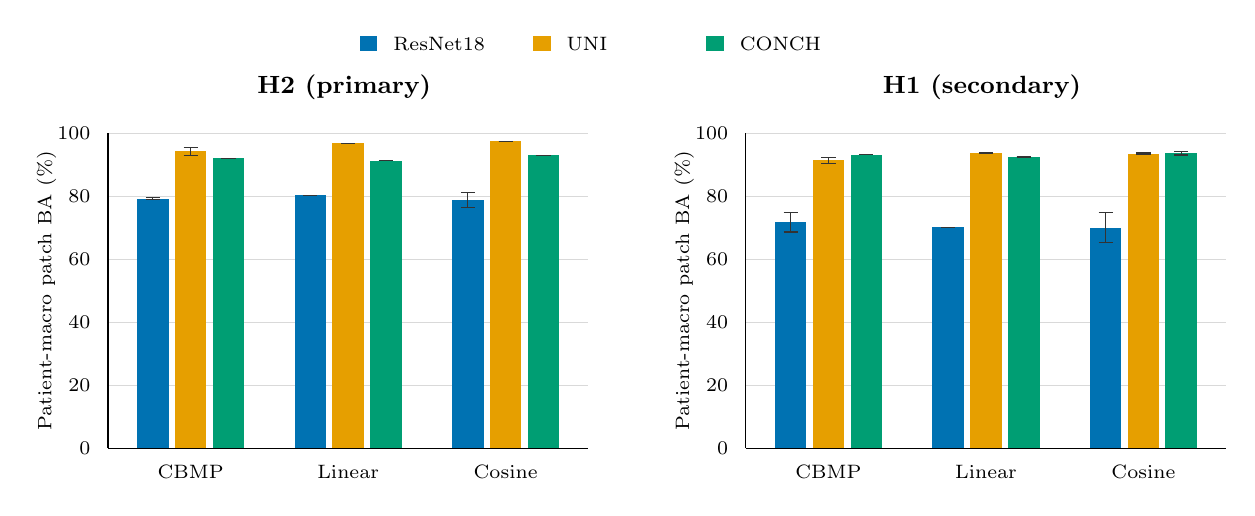
\begin{tikzpicture}[font=\scriptsize]
\definecolor{pathologyResnetBlue}{HTML}{0072B2}
\definecolor{pathologyUniOrange}{HTML}{E69F00}
\definecolor{pathologyConchGreen}{HTML}{009E73}
\fill[pathologyResnetBlue] (4.10,5.05) rectangle (4.32,5.23);
\node[anchor=west] at (4.40,5.14) {ResNet18};
\fill[pathologyUniOrange] (6.30,5.05) rectangle (6.52,5.23);
\node[anchor=west] at (6.60,5.14) {UNI};
\fill[pathologyConchGreen] (8.50,5.05) rectangle (8.72,5.23);
\node[anchor=west] at (8.80,5.14) {CONCH};
\begin{scope}[xshift=0.00cm]
\node[font=\small\bfseries] at (3.9,4.58) {H2 (primary)};
\draw[black!15] (.9,0.000) -- (7.0,0.000);
\node[anchor=east] at (.8,0.000) {0};
\draw[black!15] (.9,0.800) -- (7.0,0.800);
\node[anchor=east] at (.8,0.800) {20};
\draw[black!15] (.9,1.600) -- (7.0,1.600);
\node[anchor=east] at (.8,1.600) {40};
\draw[black!15] (.9,2.400) -- (7.0,2.400);
\node[anchor=east] at (.8,2.400) {60};
\draw[black!15] (.9,3.200) -- (7.0,3.200);
\node[anchor=east] at (.8,3.200) {80};
\draw[black!15] (.9,4.000) -- (7.0,4.000);
\node[anchor=east] at (.8,4.000) {100};
\node[rotate=90] at (.12,2) {Patient-macro patch BA (\%)};
\fill[pathologyResnetBlue] (1.270,0) rectangle (1.670,3.17150);
\draw[black!80] (1.470,3.15532) -- (1.470,3.18768);
\draw[black!80] (1.380,3.15532) -- (1.560,3.15532);
\draw[black!80] (1.380,3.18768) -- (1.560,3.18768);
\fill[pathologyUniOrange] (1.750,0) rectangle (2.150,3.76940);
\draw[black!80] (1.950,3.72146) -- (1.950,3.81734);
\draw[black!80] (1.860,3.72146) -- (2.040,3.72146);
\draw[black!80] (1.860,3.81734) -- (2.040,3.81734);
\fill[pathologyConchGreen] (2.230,0) rectangle (2.630,3.68443);
\draw[black!80] (2.430,3.68443) -- (2.430,3.68443);
\draw[black!80] (2.340,3.68443) -- (2.520,3.68443);
\draw[black!80] (2.340,3.68443) -- (2.520,3.68443);
\node at (1.950,-.30) {CBMP};
\fill[pathologyResnetBlue] (3.270,0) rectangle (3.670,3.21091);
\draw[black!80] (3.470,3.21091) -- (3.470,3.21091);
\draw[black!80] (3.380,3.21091) -- (3.560,3.21091);
\draw[black!80] (3.380,3.21091) -- (3.560,3.21091);
\fill[pathologyUniOrange] (3.750,0) rectangle (4.150,3.87129);
\draw[black!80] (3.950,3.87129) -- (3.950,3.87129);
\draw[black!80] (3.860,3.87129) -- (4.040,3.87129);
\draw[black!80] (3.860,3.87129) -- (4.040,3.87129);
\fill[pathologyConchGreen] (4.230,0) rectangle (4.630,3.65282);
\draw[black!80] (4.430,3.65282) -- (4.430,3.65282);
\draw[black!80] (4.340,3.65282) -- (4.520,3.65282);
\draw[black!80] (4.340,3.65282) -- (4.520,3.65282);
\node at (3.950,-.30) {Linear};
\fill[pathologyResnetBlue] (5.270,0) rectangle (5.670,3.15054);
\draw[black!80] (5.470,3.05401) -- (5.470,3.24707);
\draw[black!80] (5.380,3.05401) -- (5.560,3.05401);
\draw[black!80] (5.380,3.24707) -- (5.560,3.24707);
\fill[pathologyUniOrange] (5.750,0) rectangle (6.150,3.89578);
\draw[black!80] (5.950,3.89350) -- (5.950,3.89807);
\draw[black!80] (5.860,3.89350) -- (6.040,3.89350);
\draw[black!80] (5.860,3.89807) -- (6.040,3.89807);
\fill[pathologyConchGreen] (6.230,0) rectangle (6.630,3.71974);
\draw[black!80] (6.430,3.71747) -- (6.430,3.72201);
\draw[black!80] (6.340,3.71747) -- (6.520,3.71747);
\draw[black!80] (6.340,3.72201) -- (6.520,3.72201);
\node at (5.950,-.30) {Cosine};
\draw (.9,0) -- (7,0);
\draw (.9,0) -- (.9,4);
\end{scope}
\begin{scope}[xshift=8.10cm]
\node[font=\small\bfseries] at (3.9,4.58) {H1 (secondary)};
\draw[black!15] (.9,0.000) -- (7.0,0.000);
\node[anchor=east] at (.8,0.000) {0};
\draw[black!15] (.9,0.800) -- (7.0,0.800);
\node[anchor=east] at (.8,0.800) {20};
\draw[black!15] (.9,1.600) -- (7.0,1.600);
\node[anchor=east] at (.8,1.600) {40};
\draw[black!15] (.9,2.400) -- (7.0,2.400);
\node[anchor=east] at (.8,2.400) {60};
\draw[black!15] (.9,3.200) -- (7.0,3.200);
\node[anchor=east] at (.8,3.200) {80};
\draw[black!15] (.9,4.000) -- (7.0,4.000);
\node[anchor=east] at (.8,4.000) {100};
\node[rotate=90] at (.12,2) {Patient-macro patch BA (\%)};
\fill[pathologyResnetBlue] (1.270,0) rectangle (1.670,2.86932);
\draw[black!80] (1.470,2.74645) -- (1.470,2.99219);
\draw[black!80] (1.380,2.74645) -- (1.560,2.74645);
\draw[black!80] (1.380,2.99219) -- (1.560,2.99219);
\fill[pathologyUniOrange] (1.750,0) rectangle (2.150,3.65484);
\draw[black!80] (1.950,3.61478) -- (1.950,3.69490);
\draw[black!80] (1.860,3.61478) -- (2.040,3.61478);
\draw[black!80] (1.860,3.69490) -- (2.040,3.69490);
\fill[pathologyConchGreen] (2.230,0) rectangle (2.630,3.72858);
\draw[black!80] (2.430,3.72858) -- (2.430,3.72858);
\draw[black!80] (2.340,3.72858) -- (2.520,3.72858);
\draw[black!80] (2.340,3.72858) -- (2.520,3.72858);
\node at (1.950,-.30) {CBMP};
\fill[pathologyResnetBlue] (3.270,0) rectangle (3.670,2.80618);
\draw[black!80] (3.470,2.80618) -- (3.470,2.80618);
\draw[black!80] (3.380,2.80618) -- (3.560,2.80618);
\draw[black!80] (3.380,2.80618) -- (3.560,2.80618);
\fill[pathologyUniOrange] (3.750,0) rectangle (4.150,3.74981);
\draw[black!80] (3.950,3.74981) -- (3.950,3.74981);
\draw[black!80] (3.860,3.74981) -- (4.040,3.74981);
\draw[black!80] (3.860,3.74981) -- (4.040,3.74981);
\fill[pathologyConchGreen] (4.230,0) rectangle (4.630,3.69818);
\draw[black!80] (4.430,3.69818) -- (4.430,3.69818);
\draw[black!80] (4.340,3.69818) -- (4.520,3.69818);
\draw[black!80] (4.340,3.69818) -- (4.520,3.69818);
\node at (3.950,-.30) {Linear};
\fill[pathologyResnetBlue] (5.270,0) rectangle (5.670,2.80151);
\draw[black!80] (5.470,2.61208) -- (5.470,2.99094);
\draw[black!80] (5.380,2.61208) -- (5.560,2.61208);
\draw[black!80] (5.380,2.99094) -- (5.560,2.99094);
\fill[pathologyUniOrange] (5.750,0) rectangle (6.150,3.74166);
\draw[black!80] (5.950,3.73318) -- (5.950,3.75013);
\draw[black!80] (5.860,3.73318) -- (6.040,3.73318);
\draw[black!80] (5.860,3.75013) -- (6.040,3.75013);
\fill[pathologyConchGreen] (6.230,0) rectangle (6.630,3.74447);
\draw[black!80] (6.430,3.72349) -- (6.430,3.76546);
\draw[black!80] (6.340,3.72349) -- (6.520,3.72349);
\draw[black!80] (6.340,3.76546) -- (6.520,3.76546);
\node at (5.950,-.30) {Cosine};
\draw (.9,0) -- (7,0);
\draw (.9,0) -- (.9,4);
\end{scope}
\end{tikzpicture}
\caption{Equal-patient averages of patch balanced accuracy; these are not patient-diagnosis scores on the identical custom CAMELYON subset under four-candidate source-only selection. Bars show ten-seed means; whiskers show fitting-seed standard deviation, not patient- or hospital-population uncertainty. CBMP, linear logistic and trained cosine are prespecified views; all nine heads appear in the accompanying tables.}
\label{fig:pathology_encoders_patient_macro}
\end{figure*}


\subsection{Prototype audit and validation scope}
The extension reports 5,040 class-bank seed-pair comparisons: 4,828 have matching realized counts and 212 have different counts, for which no similarity is imputed. All 800 single-prototype identity checks pass, with maximum coordinate error $8.33\times10^{-16}$. The audit records 2,448 nearest-source examples. None of these checks establishes clinical semantics or independent patient linkage. The additional targeted setup/protocol/report suite contains 17 passing tests, recorded separately from the historical 44 checks. Linux execution and independent clinical semantic assessment remain unvalidated.

\subsection{Remaining validity limits}
These previously inspected hospitals provide exploratory representation comparisons. Pretraining overlap has not been independently ruled out. The original and foundation caches differ in architecture, pretraining, preprocessing and runtime, so encoder-associated differences are descriptive. Neither more seeds nor additional encoders increases patient or hospital support. Full official WILDS and new patient-linked confirmation remain separate studies.

\subsection{Prototype computational cost}
\paragraph{Cost.}
With cached $d$-dimensional features, $R$ restarts and $T$ updates cost approximately $O(RTNKd)$ for $N$ images. Stored prototypes and per-image post-encoder prediction cost $O(d\sum_cK_c)$. Encoder feature extraction is additional; prototype construction uses no gradient updates.

\subsection{Patch-level encoder comparison figure}
\begin{figure*}[t]
\centering
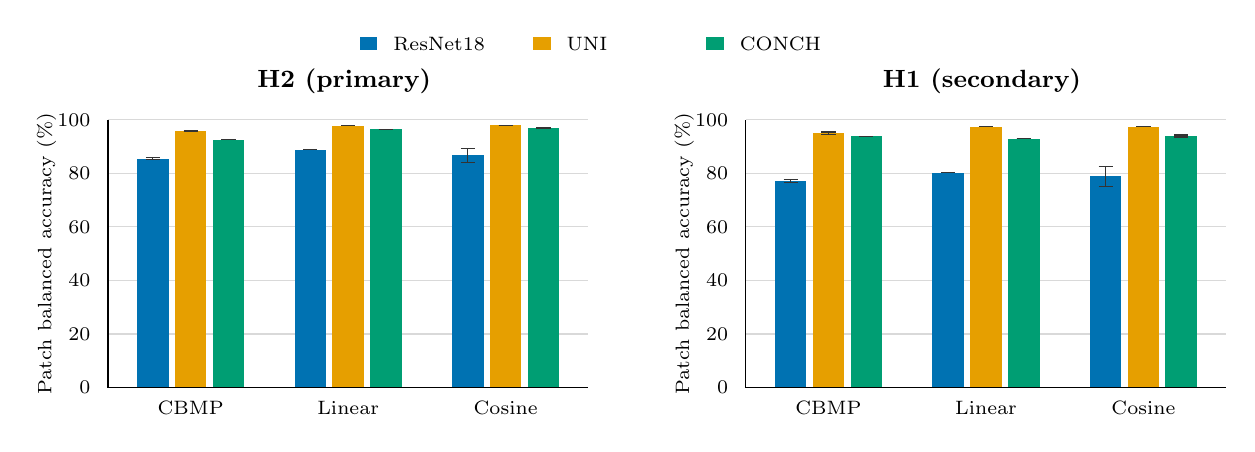
\begin{tikzpicture}[font=\scriptsize,y=.85cm]
\definecolor{pathologyResnetBlue}{HTML}{0072B2}
\definecolor{pathologyUniOrange}{HTML}{E69F00}
\definecolor{pathologyConchGreen}{HTML}{009E73}
\fill[pathologyResnetBlue] (4.10,5.05) rectangle (4.32,5.23);
\node[anchor=west] at (4.40,5.14) {ResNet18};
\fill[pathologyUniOrange] (6.30,5.05) rectangle (6.52,5.23);
\node[anchor=west] at (6.60,5.14) {UNI};
\fill[pathologyConchGreen] (8.50,5.05) rectangle (8.72,5.23);
\node[anchor=west] at (8.80,5.14) {CONCH};
\begin{scope}[xshift=0.00cm]
\node[font=\small\bfseries] at (3.9,4.58) {H2 (primary)};
\draw[black!15] (.9,0.000) -- (7.0,0.000);
\node[anchor=east] at (.8,0.000) {0};
\draw[black!15] (.9,0.800) -- (7.0,0.800);
\node[anchor=east] at (.8,0.800) {20};
\draw[black!15] (.9,1.600) -- (7.0,1.600);
\node[anchor=east] at (.8,1.600) {40};
\draw[black!15] (.9,2.400) -- (7.0,2.400);
\node[anchor=east] at (.8,2.400) {60};
\draw[black!15] (.9,3.200) -- (7.0,3.200);
\node[anchor=east] at (.8,3.200) {80};
\draw[black!15] (.9,4.000) -- (7.0,4.000);
\node[anchor=east] at (.8,4.000) {100};
\node[rotate=90] at (.12,2) {Patch balanced accuracy (\%)};
\fill[pathologyResnetBlue] (1.270,0) rectangle (1.670,3.42177);
\draw[black!80] (1.470,3.40883) -- (1.470,3.43471);
\draw[black!80] (1.380,3.40883) -- (1.560,3.40883);
\draw[black!80] (1.380,3.43471) -- (1.560,3.43471);
\fill[pathologyUniOrange] (1.750,0) rectangle (2.150,3.83201);
\draw[black!80] (1.950,3.82532) -- (1.950,3.83870);
\draw[black!80] (1.860,3.82532) -- (2.040,3.82532);
\draw[black!80] (1.860,3.83870) -- (2.040,3.83870);
\fill[pathologyConchGreen] (2.230,0) rectangle (2.630,3.70531);
\draw[black!80] (2.430,3.70531) -- (2.430,3.70531);
\draw[black!80] (2.340,3.70531) -- (2.520,3.70531);
\draw[black!80] (2.340,3.70531) -- (2.520,3.70531);
\node at (1.950,-.30) {CBMP};
\fill[pathologyResnetBlue] (3.270,0) rectangle (3.670,3.55539);
\draw[black!80] (3.470,3.55539) -- (3.470,3.55539);
\draw[black!80] (3.380,3.55539) -- (3.560,3.55539);
\draw[black!80] (3.380,3.55539) -- (3.560,3.55539);
\fill[pathologyUniOrange] (3.750,0) rectangle (4.150,3.90870);
\draw[black!80] (3.950,3.90870) -- (3.950,3.90870);
\draw[black!80] (3.860,3.90870) -- (4.040,3.90870);
\draw[black!80] (3.860,3.90870) -- (4.040,3.90870);
\fill[pathologyConchGreen] (4.230,0) rectangle (4.630,3.85998);
\draw[black!80] (4.430,3.85998) -- (4.430,3.85998);
\draw[black!80] (4.340,3.85998) -- (4.520,3.85998);
\draw[black!80] (4.340,3.85998) -- (4.520,3.85998);
\node at (3.950,-.30) {Linear};
\fill[pathologyResnetBlue] (5.270,0) rectangle (5.670,3.46901);
\draw[black!80] (5.470,3.36855) -- (5.470,3.56947);
\draw[black!80] (5.380,3.36855) -- (5.560,3.36855);
\draw[black!80] (5.380,3.56947) -- (5.560,3.56947);
\fill[pathologyUniOrange] (5.750,0) rectangle (6.150,3.91825);
\draw[black!80] (5.950,3.91540) -- (5.950,3.92109);
\draw[black!80] (5.860,3.91540) -- (6.040,3.91540);
\draw[black!80] (5.860,3.92109) -- (6.040,3.92109);
\fill[pathologyConchGreen] (6.230,0) rectangle (6.630,3.87516);
\draw[black!80] (6.430,3.87257) -- (6.430,3.87775);
\draw[black!80] (6.340,3.87257) -- (6.520,3.87257);
\draw[black!80] (6.340,3.87775) -- (6.520,3.87775);
\node at (5.950,-.30) {Cosine};
\draw (.9,0) -- (7,0);
\draw (.9,0) -- (.9,4);
\end{scope}
\begin{scope}[xshift=8.10cm]
\node[font=\small\bfseries] at (3.9,4.58) {H1 (secondary)};
\draw[black!15] (.9,0.000) -- (7.0,0.000);
\node[anchor=east] at (.8,0.000) {0};
\draw[black!15] (.9,0.800) -- (7.0,0.800);
\node[anchor=east] at (.8,0.800) {20};
\draw[black!15] (.9,1.600) -- (7.0,1.600);
\node[anchor=east] at (.8,1.600) {40};
\draw[black!15] (.9,2.400) -- (7.0,2.400);
\node[anchor=east] at (.8,2.400) {60};
\draw[black!15] (.9,3.200) -- (7.0,3.200);
\node[anchor=east] at (.8,3.200) {80};
\draw[black!15] (.9,4.000) -- (7.0,4.000);
\node[anchor=east] at (.8,4.000) {100};
\node[rotate=90] at (.12,2) {Patch balanced accuracy (\%)};
\fill[pathologyResnetBlue] (1.270,0) rectangle (1.670,3.08576);
\draw[black!80] (1.470,3.06349) -- (1.470,3.10802);
\draw[black!80] (1.380,3.06349) -- (1.560,3.06349);
\draw[black!80] (1.380,3.10802) -- (1.560,3.10802);
\fill[pathologyUniOrange] (1.750,0) rectangle (2.150,3.80071);
\draw[black!80] (1.950,3.78366) -- (1.950,3.81776);
\draw[black!80] (1.860,3.78366) -- (2.040,3.78366);
\draw[black!80] (1.860,3.81776) -- (2.040,3.81776);
\fill[pathologyConchGreen] (2.230,0) rectangle (2.630,3.75163);
\draw[black!80] (2.430,3.75163) -- (2.430,3.75163);
\draw[black!80] (2.340,3.75163) -- (2.520,3.75163);
\draw[black!80] (2.340,3.75163) -- (2.520,3.75163);
\node at (1.950,-.30) {CBMP};
\fill[pathologyResnetBlue] (3.270,0) rectangle (3.670,3.21201);
\draw[black!80] (3.470,3.21201) -- (3.470,3.21201);
\draw[black!80] (3.380,3.21201) -- (3.560,3.21201);
\draw[black!80] (3.380,3.21201) -- (3.560,3.21201);
\fill[pathologyUniOrange] (3.750,0) rectangle (4.150,3.89895);
\draw[black!80] (3.950,3.89895) -- (3.950,3.89895);
\draw[black!80] (3.860,3.89895) -- (4.040,3.89895);
\draw[black!80] (3.860,3.89895) -- (4.040,3.89895);
\fill[pathologyConchGreen] (4.230,0) rectangle (4.630,3.71525);
\draw[black!80] (4.430,3.71525) -- (4.430,3.71525);
\draw[black!80] (4.340,3.71525) -- (4.520,3.71525);
\draw[black!80] (4.340,3.71525) -- (4.520,3.71525);
\node at (3.950,-.30) {Linear};
\fill[pathologyResnetBlue] (5.270,0) rectangle (5.670,3.15606);
\draw[black!80] (5.470,3.00466) -- (5.470,3.30745);
\draw[black!80] (5.380,3.00466) -- (5.560,3.00466);
\draw[black!80] (5.380,3.30745) -- (5.560,3.30745);
\fill[pathologyUniOrange] (5.750,0) rectangle (6.150,3.89918);
\draw[black!80] (5.950,3.89708) -- (5.950,3.90129);
\draw[black!80] (5.860,3.89708) -- (6.040,3.89708);
\draw[black!80] (5.860,3.90129) -- (6.040,3.90129);
\fill[pathologyConchGreen] (6.230,0) rectangle (6.630,3.75816);
\draw[black!80] (6.430,3.74296) -- (6.430,3.77335);
\draw[black!80] (6.340,3.74296) -- (6.520,3.74296);
\draw[black!80] (6.340,3.77335) -- (6.520,3.77335);
\node at (5.950,-.30) {Cosine};
\draw (.9,0) -- (7,0);
\draw (.9,0) -- (.9,4);
\end{scope}
\end{tikzpicture}
\caption{Patch-level balanced accuracy on the identical custom CAMELYON subset under four-candidate source-only selection. Bars show ten-seed means; whiskers show fitting-seed standard deviation, not patient- or hospital-population uncertainty. CBMP, linear logistic and trained cosine are prespecified views; all nine heads appear in the accompanying tables.}
\label{fig:pathology_encoders_patch}
\end{figure*}


\section{Limits and further validation protocol}
Earlier threshold and sequence-removal diagnostics used three fitting seeds and remain versioned separately from the current ten-seed results. The removal analysis resampled observational source cohorts: dominant-center removal and approximately proportional scarcity matching preserve class coverage but can differ in frames and prevalence. It is inconclusive evidence about imbalance and is distinct from the algorithmic K-by-beta factorial. No controlled generative simulation or causal clinical mechanism is established.

The cohort, patient identities, primary contrasts and tuning rules should be frozen before testing a new independent cohort. A mechanism contrast is beta 1 versus 0 at $K=4$, with Across AUROC and BA reported together. Positive-bearing and negative-only independent examinations are necessary for sequence inference; clinical patient/slide endpoints need separate labels. Hospital-population inference requires a suitable sampling design and more independent hospitals, not additional patches at the same sites. Rotating the five inspected WILDS hospitals would remain an exploratory custom protocol.

The optional official-split adapter uses complete WILDS indices/evaluator, H0/H3/H4 training, H1 validation without refitting, H2 testing and ten seeds. External pretraining defines a non-standard setting under WILDS rules~\cite{wilds2026submission}. Prior H2 inspection remains disclosed. Original UNI and CONCH adapters record checkpoint hash, exact revision, preprocessing and feature definition~\cite{chen2024uni,lu2024conch}. Original UNI and CONCH provider/checkpoint integration and custom-cohort comparisons are now complete. Full official evaluation, modern DG training baselines and a new patient-linked cohort remain unexecuted. The released development protocol specifies those prerequisites without reporting them as completed experiments.

\bibliographystyle{ieeenat_fullname}
\bibliography{main}
\end{document}
